\documentclass[11pt, twoside, openany]{book}
\usepackage[margin=0.5in]{geometry}
\usepackage{graphicx}
\usepackage{multicol}
\setlength{\parindent}{0pt}
\title{ \LARGE \textbf{Dunn Family Recipe Book}}
\begin{document}
\maketitle
\section*{Table of Contents}
{~\vspace{2mm}\\ \Large \textbf{Appetizers}}\hfill\textbf{\pageref{appetizers}}

Black Bean and Corn Salsa\hrulefill\pageref{black-bean-and-corn-salsa}\\
Bunco Bites\hrulefill\pageref{bunco-bites}\\
Chicken Wing Dip\hrulefill\pageref{chicken-wing-dip}\\
Crab Appetizers\hrulefill\pageref{crab-appetizers}\\
Jalapeno Poppers\hrulefill\pageref{jalapeno-poppers}\\
Power Balls\hrulefill\pageref{power-balls}\\
Pumpkin Dip\hrulefill\pageref{pumpkin-dip}\\
Spinach Balls\hrulefill\pageref{spinach-balls}\\
{~\vspace{2mm}\\ \Large \textbf{Salads}}\hfill\textbf{\pageref{salads}}

Apple, Dried Cherry, and Walnut Salad Base\hrulefill\pageref{apple,-dried-cherry,-and-walnut-salad-base}\\
Apple, Dried Cherry, and Walnut Salad Maple Dressing\hrulefill\pageref{apple,-dried-cherry,-and-walnut-salad-maple-dressing}\\
French Potato Salad\hrulefill\pageref{french-potato-salad}\\
Oriental Chicken Salad\hrulefill\pageref{oriental-chicken-salad}\\
Strawberry Salad with Poppy Seed Dressing\hrulefill\pageref{strawberry-salad-with-poppy-seed-dressing}\\
{~\vspace{2mm}\\ \Large \textbf{Soups}}\hfill\textbf{\pageref{soups}}

Butternut Squash Bisque\hrulefill\pageref{butternut-squash-bisque}\\
Chicken Taco Stew\hrulefill\pageref{chicken-taco-stew}\\
Corn Chowder\hrulefill\pageref{corn-chowder}\\
Egg Drop Soup\hrulefill\pageref{egg-drop-soup}\\
Potato Leek Soup\hrulefill\pageref{potato-leek-soup}\\
Spicy White Turkey Chili Soup\hrulefill\pageref{spicy-white-turkey-chili-soup}\\
{~\vspace{2mm}\\ \Large \textbf{Sides}}\hfill\textbf{\pageref{sides}}

Blueberry Muffins\hrulefill\pageref{blueberry-muffins}\\
Sweet Potatoes Mashed\hrulefill\pageref{sweet-potatoes-mashed}\\
{~\vspace{2mm}\\ \Large \textbf{Breakfasts}}\hfill\textbf{\pageref{breakfasts}}

Ham and Broccoli Casserole\hrulefill\pageref{ham-and-broccoli-casserole}\\
Pancakes\hrulefill\pageref{pancakes}\\
Pumpkin Waffles\hrulefill\pageref{pumpkin-waffles}\\
{~\vspace{2mm}\\ \Large \textbf{Dips}}\hfill\textbf{\pageref{dips}}

Pumpkin Dip\hrulefill\pageref{pumpkin-dip}\\
{~\vspace{2mm}\\ \Large \textbf{Seafood}}\hfill\textbf{\pageref{seafood}}

Bourbon Bacon Scallops\hrulefill\pageref{bourbon-bacon-scallops}\\
Coconut Shrimp\hrulefill\pageref{coconut-shrimp}\\
Crab Casserole\hrulefill\pageref{crab-casserole}\\
Honey Balsamic Salmon\hrulefill\pageref{honey-balsamic-salmon}\\
Pan-Seared Scallops\hrulefill\pageref{pan-seared-scallops}\\
{~\vspace{2mm}\\ \Large \textbf{Steak}}\hfill\textbf{\pageref{steak}}

Steak Teriyaki Marinade\hrulefill\pageref{steak-teriyaki-marinade}\\
{~\vspace{2mm}\\ \Large \textbf{Pork}}\hfill\textbf{\pageref{pork}}

Barbecue Sauce\hrulefill\pageref{barbecue-sauce}\\
Rib Sauce\hrulefill\pageref{rib-sauce}\\
Sausage Balls\hrulefill\pageref{sausage-balls}\\
Southern Succor Rub\hrulefill\pageref{southern-succor-rub}\\
{~\vspace{2mm}\\ \Large \textbf{Chicken}}\hfill\textbf{\pageref{chicken}}

Broccoli Chicken Casserole\hrulefill\pageref{broccoli-chicken-casserole}\\
Chicken Cordon Bleu\hrulefill\pageref{chicken-cordon-bleu}\\
Chicken Devan\hrulefill\pageref{chicken-devan}\\
Chicken Enchiladas\hrulefill\pageref{chicken-enchiladas}\\
Chicken and Artichoke Bake\hrulefill\pageref{chicken-and-artichoke-bake}\\
Chile, Chicken, and Cheese Casserole\hrulefill\pageref{chile,-chicken,-and-cheese-casserole}\\
Cream Cheese Spinach Stuffed Chicken\hrulefill\pageref{cream-cheese-spinach-stuffed-chicken}\\
Oriental Chicken Salad\hrulefill\pageref{oriental-chicken-salad}\\
Seared Chicken With Avocado\hrulefill\pageref{seared-chicken-with-avocado}\\
Sour Cream Salsa Chicken\hrulefill\pageref{sour-cream-salsa-chicken}\\
{~\vspace{2mm}\\ \Large \textbf{Pastas}}\hfill\textbf{\pageref{pastas}}

Cauliflower Casserole\hrulefill\pageref{cauliflower-casserole}\\
Mac and Cheese\hrulefill\pageref{mac-and-cheese}\\
Spaghetti Squash Gratin\hrulefill\pageref{spaghetti-squash-gratin}\\
{~\vspace{2mm}\\ \Large \textbf{Breads}}\hfill\textbf{\pageref{breads}}

Amish Cinnamon Bread\hrulefill\pageref{amish-cinnamon-bread}\\
Apple Wheat Bread\hrulefill\pageref{apple-wheat-bread}\\
Banana Bread\hrulefill\pageref{banana-bread}\\
Zucchini Bread\hrulefill\pageref{zucchini-bread}\\
{~\vspace{2mm}\\ \Large \textbf{Pies}}\hfill\textbf{\pageref{pies}}

Grasshopper Pie\hrulefill\pageref{grasshopper-pie}\\
Pizza Bites\hrulefill\pageref{pizza-bites}\\
{~\vspace{2mm}\\ \Large \textbf{Cookies}}\hfill\textbf{\pageref{cookies}}

Almond Macaroons\hrulefill\pageref{almond-macaroons}\\
Chocolate Chip Cookies\hrulefill\pageref{chocolate-chip-cookies}\\
Christmas Crackle\hrulefill\pageref{christmas-crackle}\\
Cookies and Cream Oreo Bark\hrulefill\pageref{cookies-and-cream-oreo-bark}\\
Mint Meringues Recipe\hrulefill\pageref{mint-meringues-recipe}\\
Monster Cookies\hrulefill\pageref{monster-cookies}\\
Peanut Butter Balls\hrulefill\pageref{peanut-butter-balls}\\
Peanut Butter Blossoms\hrulefill\pageref{peanut-butter-blossoms}\\
Peanut Butter Cookies\hrulefill\pageref{peanut-butter-cookies}\\
Peppermint Bark\hrulefill\pageref{peppermint-bark}\\
Russian Tea Cakes\hrulefill\pageref{russian-tea-cakes}\\
{~\vspace{2mm}\\ \Large \textbf{Cakes}}\hfill\textbf{\pageref{cakes}}

Angel Food Cake Base\hrulefill\pageref{angel-food-cake-base}\\
Angel Food Cake Strawberry Sauce\hrulefill\pageref{angel-food-cake-strawberry-sauce}\\
Apple Cake\hrulefill\pageref{apple-cake}\\
Chocolate Chip Cheesecake\hrulefill\pageref{chocolate-chip-cheesecake}\\
Devil's Food Cake\hrulefill\pageref{devil's-food-cake}\\
French Almond Cake\hrulefill\pageref{french-almond-cake}\\
Mini Cheesecakes\hrulefill\pageref{mini-cheesecakes}\\
Sour Cream Coffee Cake\hrulefill\pageref{sour-cream-coffee-cake}\\
{~\vspace{2mm}\\ \Large \textbf{Desserts}}\hfill\textbf{\pageref{desserts}}

Blueberry Kuchen\hrulefill\pageref{blueberry-kuchen}\\
Blueberry Maple Muffins\hrulefill\pageref{blueberry-maple-muffins}\\
Chocolate Almond Mousse\hrulefill\pageref{chocolate-almond-mousse}\\
Chocolate Brownies\hrulefill\pageref{chocolate-brownies}\\
Chocolate Chip Muffins\hrulefill\pageref{chocolate-chip-muffins}\\
Dark Chocolate Brownies\hrulefill\pageref{dark-chocolate-brownies}\\
Flourless Chocolate Torte\hrulefill\pageref{flourless-chocolate-torte}\\
Fudge\hrulefill\pageref{fudge}\\
Island Gem Bars\hrulefill\pageref{island-gem-bars}\\
No Bake Brownies\hrulefill\pageref{no-bake-brownies}\\
Oreo Truffles\hrulefill\pageref{oreo-truffles}\\
Pecan Tassies\hrulefill\pageref{pecan-tassies}\\
Raspberry Crisp\hrulefill\pageref{raspberry-crisp}\\
Rock Candy\hrulefill\pageref{rock-candy}\\
Sticky Buns\hrulefill\pageref{sticky-buns}\\
{\newpage \LARGE \textbf{Appetizers}} \label{appetizers}\\
\noindent\begin{minipage}[t]{\linewidth}%
{\Large\textbf{Black Bean and Corn Salsa}} \label{black-bean-and-corn-salsa}\hfill\textit{Sue Dunn}\\
\noindent\begin{minipage}[t]{0.78\linewidth}%
\textbf{Ingredients}:\vspace{-3mm}
\begin{multicols}{2}
\begin{itemize}\setlength\itemsep{-1mm}
\item 15 oz can black beans, rinsed and drained
\item 11 oz can whole kernel corn, drained
\item 1 tsp minced fresh jalepeno pepper (optional)
\item 1 avacado, chopped
\item 2 medium tomatoes, chopped
\item 1 red bell pepper, chopped
\item 1/3 cup chopped fresh cilantro (or substitute 1 tsp dried cilantro)
\item 1/4 cup diced red onion
\item 1/4 cup fresh lime juice (about 2 limes, squeezed)
\item 1 tsp salt
\item tortilla chips for dipping (scoop chips work best)
\end{itemize}
\end{multicols}
\end{minipage}
\noindent\begin{minipage}[t]{0.18\linewidth}
\centering \strut\vspace*{-\baselineskip}\newline
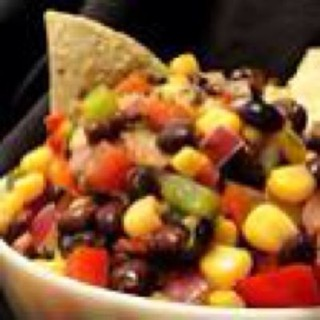
\includegraphics[width=0.9\linewidth]{/home/tim/Documents/projects/recipes/img/D16A291D-6D83-4C6F-BB6B-8E1E1CDA99D5.jpg}\\
\end{minipage}\vspace{3mm}
\textbf{Directions}:
\vspace{-3mm}\begin{enumerate}\setlength\itemsep{-1mm}
\item Combine all ingredients except avocado and chips. Cover and chill for at least 2 hours. Add avacodo just before serving. Serve with chips.
\end{enumerate}
\end{minipage}\vspace{8mm}
\noindent\begin{minipage}[t]{\linewidth}%
{\Large\textbf{Bunco Bites}} \label{bunco-bites}\hfill\textit{Mary Reynolds}\\
\noindent\begin{minipage}[t]{0.78\linewidth}%
\textbf{Ingredients}:\vspace{-3mm}
\begin{multicols}{2}
\begin{itemize}\setlength\itemsep{-1mm}
\item mini square party pretzels
\item M and Ms
\item white chocolate wafers
\end{itemize}
\end{multicols}
\end{minipage}
\noindent\begin{minipage}[t]{0.18\linewidth}
\centering \strut\vspace*{-\baselineskip}\newline
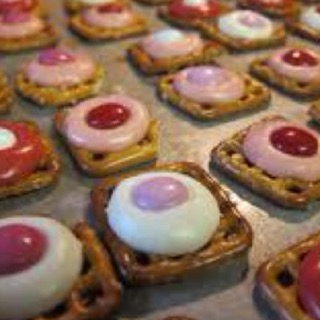
\includegraphics[width=0.9\linewidth]{/home/tim/Documents/projects/recipes/img/E80AF034-6CDF-4993-A223-474B6DFBA2BA.jpg}\\
\end{minipage}\vspace{3mm}
\textbf{Directions}:
\vspace{-3mm}\begin{enumerate}\setlength\itemsep{-1mm}
\item Preheat oven to 225F. Place single layer of pretzels on cookie sheet. Place one wafer on center of each pretzel. Warm in oven for 3-5 minutes to soften wafer. Remove from oven and place one M and M in center of each wafer. Cool in fridge until wafer hardens.
\end{enumerate}
\end{minipage}\vspace{8mm}
\noindent\begin{minipage}[t]{\linewidth}%
{\Large\textbf{Chicken Wing Dip}} \label{chicken-wing-dip}\hfill\textit{Tom Dunn}\\
\noindent\begin{minipage}[t]{0.78\linewidth}%
\textbf{Ingredients}:\vspace{-3mm}
\begin{multicols}{2}
\begin{itemize}\setlength\itemsep{-1mm}
\item 4-6 oz Frank's original Hot sauce
\item 2 (8 oz) packages regular (not low fat) cream cheese
\item 8 oz bottle ranch or bleu cheese salad dressing
\item 2 cups cooked shredded chicken
\item 8 oz shredded monterey jack or cheddar cheese
\end{itemize}
\end{multicols}
\end{minipage}
\noindent\begin{minipage}[t]{0.18\linewidth}
\centering \strut\vspace*{-\baselineskip}\newline
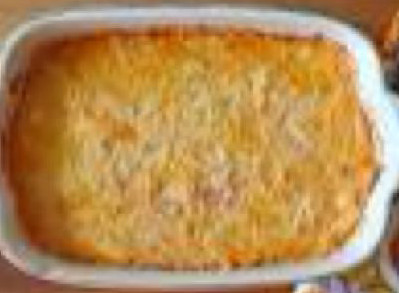
\includegraphics[width=0.9\linewidth]{/home/tim/Documents/projects/recipes/img/31362A38-BD46-4715-9B26-0AC1C3991F65.jpg}\\
\end{minipage}\vspace{3mm}
\textbf{Directions}:
\vspace{-3mm}\begin{enumerate}\setlength\itemsep{-1mm}
\item Cook and shred chicken.
\item In a medium-size saucepan, bring hot sauce to a simmer over medium-low heat. Add cream cheese and stir continuously until fully melted. Stir in dressing.
\item Add chicken and stir until fully coated. Add shredded cheese and stir until fully melted.
\item Transfer mixture to a small crockpot and heat on low. Or transfer to a small casserole dish and bake at 350F until bubbly (20-25 minutes). 
\item Serve warm with tortilla chips.
\end{enumerate}
\end{minipage}\vspace{8mm}
\noindent\begin{minipage}[t]{\linewidth}%
{\Large\textbf{Crab Appetizers}} \label{crab-appetizers}\hfill\textit{Barb McKinley}\\
\textbf{Yield:} \textit{makes 24}\\
\noindent\begin{minipage}[t]{0.78\linewidth}%
\textbf{Ingredients}:\vspace{-3mm}
\begin{multicols}{2}
\begin{itemize}\setlength\itemsep{-1mm}
\item 1 can (7 oz) of crab meat (Fancy Lump)
\item 1 stick of butter, softened
\item 1 jar (5 oz) Kraft Old English Cheese
\item 1/2 tsp garlic powder
\item 2 tsp mayonnaise
\item 6 English muffins
\end{itemize}
\end{multicols}
\end{minipage}
\noindent\begin{minipage}[t]{0.18\linewidth}
\centering \strut\vspace*{-\baselineskip}\newline

\includegraphics[width=0.9\linewidth]{/home/tim/Documents/projects/recipes/img/none.jpg}\\
\end{minipage}\vspace{3mm}
\textbf{Directions}:
\vspace{-3mm}\begin{enumerate}\setlength\itemsep{-1mm}
\item Open English muffins, then cut in half again, making 24 quarter pieces. Wash the crab meat, looking for loose pieces of shell.
\item Mix all ingredients together and place atop English muffins.
\item Bake for 20 minutes at 400F.
\end{enumerate}
\end{minipage}\vspace{8mm}
\noindent\begin{minipage}[t]{\linewidth}%
{\Large\textbf{Jalapeno Poppers}} \label{jalapeno-poppers}\hfill\textit{Trey Dunn}\\
\textbf{Yield:} \textit{makes 24 peppers}\\
\noindent\begin{minipage}[t]{0.78\linewidth}%
\textbf{Ingredients}:\vspace{-3mm}
\begin{multicols}{2}
\begin{itemize}\setlength\itemsep{-1mm}
\item 12 jalapeno peppers, cut in half and seeded
\item 2 packages of cream cheese
\item 1.5 lb bacon (Wright)
\item 2 handfuls sharp cheddar cheese
\item garlic powder
\end{itemize}
\end{multicols}
\end{minipage}
\noindent\begin{minipage}[t]{0.18\linewidth}
\centering \strut\vspace*{-\baselineskip}\newline

\includegraphics[width=0.9\linewidth]{/home/tim/Documents/projects/recipes/img/none.jpg}\\
\end{minipage}\vspace{3mm}
\textbf{Directions}:
\vspace{-3mm}\begin{enumerate}\setlength\itemsep{-1mm}
\item Heat oven to 400F. Prepare peppers.
\item Heat cream cheese in microwave until soft (30 seconds). Add cheddar cheese and garlic powder. Combine, and add the mixture into the peppers, filling them to the top.
\item Cut the bacon strips in half and wrap around the pepper, securing with a toothpick. Cook for about 30 minutes or until done.
\end{enumerate}
\end{minipage}\vspace{8mm}
\noindent\begin{minipage}[t]{\linewidth}%
{\Large\textbf{Power Balls}} \label{power-balls}\hfill\textit{Sue Dunn}\\
\noindent\begin{minipage}[t]{0.78\linewidth}%
\textbf{Ingredients}:\vspace{-3mm}
\begin{multicols}{2}
\begin{itemize}\setlength\itemsep{-1mm}
\item 2 cups oatmeal
\item 1/2 cup peanut butter
\item 1/3 cup honey
\item 1/2 cup chocolate chips
\item 1 tsp vanilla
\item 1/8 cup ground flax seed
\end{itemize}
\end{multicols}
\end{minipage}
\noindent\begin{minipage}[t]{0.18\linewidth}
\centering \strut\vspace*{-\baselineskip}\newline
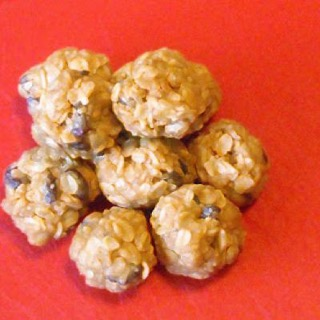
\includegraphics[width=0.9\linewidth]{/home/tim/Documents/projects/recipes/img/881F7E37-ABBD-497D-A638-12EFC9985D4A.jpg}\\
\end{minipage}\vspace{3mm}
\textbf{Directions}:
\vspace{-3mm}\begin{enumerate}\setlength\itemsep{-1mm}
\item In a large mixing bowl, add together the dry ingredients (oatmeal, flax seed, chocolate chips). Mix together.
\item Add in peanut butter, honey, and vanilla. Mix together thoroughly. Refrigerate to make your dough a bit firmer.
\item Roll bits of dough into 1 inch balls. Place in an air tight container and store in the refrigerator. They can be stored for up to one week.
\end{enumerate}
\end{minipage}\vspace{8mm}
\noindent\begin{minipage}[t]{\linewidth}%
{\Large\textbf{Pumpkin Dip}} \label{pumpkin-dip}\hfill\textit{Donna Knights}\\
\textit{``Half of this recipe is usually enough''}\\
\noindent\begin{minipage}[t]{0.78\linewidth}%
\textbf{Ingredients}:\vspace{-3mm}
\begin{multicols}{2}
\begin{itemize}\setlength\itemsep{-1mm}
\item 2 cups confectioners sugar
\item 8 oz cream cheese, softened
\item 15 oz canned pumpkin
\item 1 tsp cinnamon
\item 1/2 tsp ginger
\item 1 dash nutmeg
\end{itemize}
\end{multicols}
\end{minipage}
\noindent\begin{minipage}[t]{0.18\linewidth}
\centering \strut\vspace*{-\baselineskip}\newline
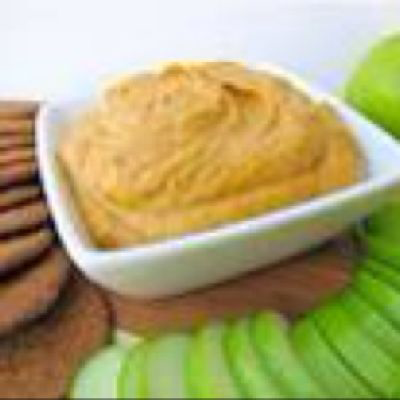
\includegraphics[width=0.9\linewidth]{/home/tim/Documents/projects/recipes/img/B96CF91B-E4BA-4702-A0BA-1BDE96A6206A.jpg}\\
\end{minipage}\vspace{3mm}
\textbf{Directions}:
\vspace{-3mm}\begin{enumerate}\setlength\itemsep{-1mm}
\item Beat all ingredients until smooth, and refrigerate.
\item Serve with ginger snaps/apples, etc.
\end{enumerate}
\end{minipage}\vspace{8mm}
\noindent\begin{minipage}[t]{\linewidth}%
{\Large\textbf{Spinach Balls}} \label{spinach-balls}\hfill\textit{Sue Dunn}\\
\noindent\begin{minipage}[t]{0.78\linewidth}%
\textbf{Ingredients}:\vspace{-3mm}
\begin{multicols}{2}
\begin{itemize}\setlength\itemsep{-1mm}
\item 1 (10 oz) package frozen chopped spinach, thawed and drained
\item 2 cups finely crushed herb-seasoned dry bread stuffing mix
\item 1/2 cup grated parmesan cheese
\item 2 tsp garlic powder
\item 1/2 tsp ground black pepper
\item 1 tsp italian seasoning
\item 1/4 cup melted butter
\item 3 eggs, beaten
\item 3/4 cup chopped onions
\end{itemize}
\end{multicols}
\end{minipage}
\noindent\begin{minipage}[t]{0.18\linewidth}
\centering \strut\vspace*{-\baselineskip}\newline
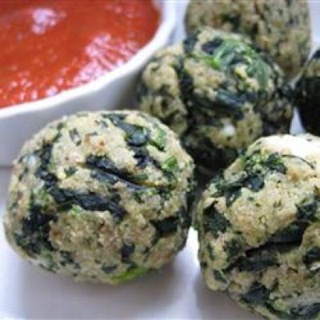
\includegraphics[width=0.9\linewidth]{/home/tim/Documents/projects/recipes/img/13577261-2CCD-4BCD-BD18-734529F16541.jpg}\\
\end{minipage}\vspace{3mm}
\textbf{Directions}:
\vspace{-3mm}\begin{enumerate}\setlength\itemsep{-1mm}
\item Preheat oven to 350F.
\item In a large bowl, combine spinach, stuffing mix, Parmesan cheese, garlic powder, black pepper, Italian seasoning, melted butter, eggs, and onions. Shape into walnut-sized balls and place on a baking sheet.
\item Bake for 20 minutes, or until lightly browned.
\end{enumerate}
\end{minipage}\vspace{8mm}

{\newpage \LARGE \textbf{Salads}} \label{salads}\\
\noindent\begin{minipage}[t]{\linewidth}%
{\Large\textbf{Apple, Dried Cherry, and Walnut Salad Base}} \label{apple,-dried-cherry,-and-walnut-salad-base}\hfill\textit{Linda Garner}\\
\textit{``With maple dressing (next recipe)''}\\
\textbf{Yield:} \textit{serves 6}\\
\noindent\begin{minipage}[t]{0.78\linewidth}%
\textbf{Ingredients}:\vspace{-3mm}
\begin{multicols}{2}
\begin{itemize}\setlength\itemsep{-1mm}
\item 5oz bag mixed baby greens (10 cups lightly packed
\item 2 Granny Smith apples
\item 1/2 cup dried tart cherries
\item 1/2 cup chopped walnuts, toasted
\item 1/4 cup crumbled Maytag bleu cheese
\end{itemize}
\end{multicols}
\end{minipage}
\noindent\begin{minipage}[t]{0.18\linewidth}
\centering \strut\vspace*{-\baselineskip}\newline

\includegraphics[width=0.9\linewidth]{/home/tim/Documents/projects/recipes/img/none.jpg}\\
\end{minipage}\vspace{3mm}
\textbf{Directions}:
\vspace{-3mm}\begin{enumerate}\setlength\itemsep{-1mm}
\item Peel and core apples. Chop into matchstick-sized strips.
\item Toss greens, apples, cherries, and 1/4 cup walnuts in large bowl to combine. Toss with enough dressing to coat. Divide salad equally among all plates. Sprinkle remaining 1/4 cup walnuts and serve.
\end{enumerate}
\end{minipage}\vspace{8mm}
\noindent\begin{minipage}[t]{\linewidth}%
{\Large\textbf{Apple, Dried Cherry, and Walnut Salad Maple Dressing}} \label{apple,-dried-cherry,-and-walnut-salad-maple-dressing}\hfill\textit{Linda Garner}\\
\textit{``Dressing can be prepared up to 3 days ahead. Cover and refrigerate. Re-whisk before using.''}\\
\noindent\begin{minipage}[t]{0.78\linewidth}%
\textbf{Ingredients}:\vspace{-3mm}
\begin{multicols}{2}
\begin{itemize}\setlength\itemsep{-1mm}
\item 1/4 cup mayonnaise
\item 1/4 cup pure maple syrup
\item 3 Tbsp Champagne/white vinegar
\item 2 tsp sugar
\item 1/2 cup vegetable oil
\end{itemize}
\end{multicols}
\end{minipage}
\noindent\begin{minipage}[t]{0.18\linewidth}
\centering \strut\vspace*{-\baselineskip}\newline

\includegraphics[width=0.9\linewidth]{/home/tim/Documents/projects/recipes/img/none.jpg}\\
\end{minipage}\vspace{3mm}
\textbf{Directions}:
\vspace{-3mm}\begin{enumerate}\setlength\itemsep{-1mm}
\item Whisk mayonnaise, maple syrup, vinegar, and sugar in medium bowl to blend.
\item Gradually whisk in oil until mixture thickens slightly. Season to taste with salt and pepper.
\end{enumerate}
\end{minipage}\vspace{8mm}
\noindent\begin{minipage}[t]{\linewidth}%
{\Large\textbf{French Potato Salad}} \label{french-potato-salad}\hfill\textit{Sue Dunn}\\
\textbf{Yield:} \textit{4-6 servings}\\
\noindent\begin{minipage}[t]{0.78\linewidth}%
\textbf{Ingredients}:\vspace{-3mm}
\begin{multicols}{2}
\begin{itemize}\setlength\itemsep{-1mm}
\item 1 lb small white boiling potatoes
\item 1 lb small red boiling potatoes
\item 2 Tbsp dry white wine
\item 2 Tbsp chicken stock
\item 3 Tbsp vinegar
\item 1/2 tsp Dijon mustard
\item 2 tsp kosher salt
\item 3/4 tsp ground black pepper
\item 10 Tbsp olive oil
\item 1/4 cup minced scallions
\item 2 Tbsp minced fresh dill
\item 2 Tbsp minced parsley
\item 2 Tbsp minced basil
\end{itemize}
\end{multicols}
\end{minipage}
\noindent\begin{minipage}[t]{0.18\linewidth}
\centering \strut\vspace*{-\baselineskip}\newline
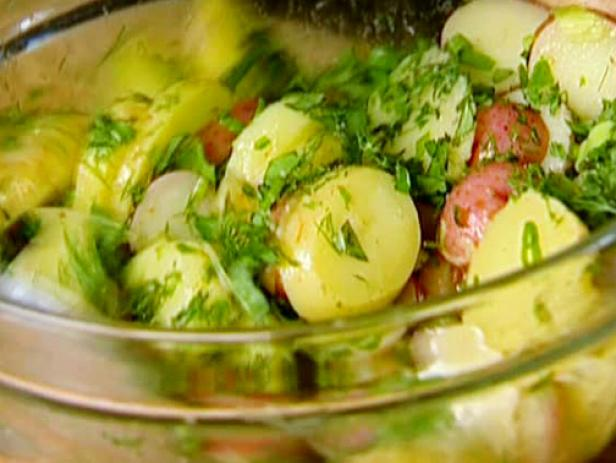
\includegraphics[width=0.9\linewidth]{/home/tim/Documents/projects/recipes/img/potato_salad.jpg}\\
\end{minipage}\vspace{3mm}
\textbf{Directions}:
\vspace{-3mm}\begin{enumerate}\setlength\itemsep{-1mm}
\item Cook the white and red potatoes in a large boiling pot of salted water for 20-30 minutes, until cooked through. Drain and place a towel over them, allowing them to steam for 10 more minutes. As soon as you can handle them, cut in half (or smaller) and place in a medium bowl. Toss gently with the wine and chicken stock. Alow the liquids to soak into the warm potatoes before proceeding.
\item Combine the vinegar, mustard, 1/2 tsp salt, 1/4 tsp pepper and slowly whisk in the olive oil to make an emulsion. Add the vinaigrette to the potatoes. Add the scallions, dill, parsley, basil, 1 1/2 tsp salt, and 1/2 tsp pepper and toss. Serve warm or at room temperature.
\end{enumerate}
\end{minipage}\vspace{8mm}
\noindent\begin{minipage}[t]{\linewidth}%
{\Large\textbf{Strawberry Salad with Poppy Seed Dressing}} \label{strawberry-salad-with-poppy-seed-dressing}\hfill\textit{Sue Dunn}\\
\textbf{Yield:} \textit{Serves 6}\\
\noindent\begin{minipage}[t]{0.78\linewidth}%
\textbf{Ingredients}:\vspace{-3mm}
\begin{multicols}{2}
\begin{itemize}\setlength\itemsep{-1mm}
\item 3 Tbsp sugar
\item 3 Tbsp mayonnaise
\item 2 Tbsp milk
\item 1 Tbsp poppy seeds
\item 1 Tbsp white wine vinegar
\item 1 bag (10 oz) romaine lettuce
\item 1 cup strawberries, sliced
\item 2 Tbsp toasted slivered almonds
\end{itemize}
\end{multicols}
\end{minipage}
\noindent\begin{minipage}[t]{0.18\linewidth}
\centering \strut\vspace*{-\baselineskip}\newline

\includegraphics[width=0.9\linewidth]{/home/tim/Documents/projects/recipes/img/none.jpg}\\
\end{minipage}\vspace{3mm}
\textbf{Directions}:
\vspace{-3mm}\begin{enumerate}\setlength\itemsep{-1mm}
\item Combine first 5 ingredients in a small bowl, stirring with a whisk. Place lettuce in a large bowl; add strawberries and almonds, tossing to combine. Divide salad among 6 plates. Drizzle 1 Tbsp dressing over each serving.
\end{enumerate}
\end{minipage}\vspace{8mm}

{\newpage \LARGE \textbf{Soups}} \label{soups}\\
\noindent\begin{minipage}[t]{\linewidth}%
{\Large\textbf{Butternut Squash Bisque}} \label{butternut-squash-bisque}\hfill\textit{Sue Dunn}\\
\textbf{Yield:} \textit{Serves 6}\\
\noindent\begin{minipage}[t]{0.78\linewidth}%
\textbf{Ingredients}:\vspace{-3mm}
\begin{multicols}{2}
\begin{itemize}\setlength\itemsep{-1mm}
\item 2 tsp unsalted butter
\item 1 1/2 cup onion, chopped
\item 1 1/2 tsp kosher salt
\item 2 tsp minced garlic
\item 1 pinch ground nutmeg
\item 1 pinch cayenne pepper
\item 4 lbs uncooked butternut squash, cubed
\item 4 cups reduced-sodium chicken/vegetable broth
\item 3 Tbsp plain low fat Greek yogurt
\item 1 Tbsp packed light brown sugar
\item 2 tsp fresh sage, chopped
\item 1/4 tsp black pepper
\end{itemize}
\end{multicols}
\end{minipage}
\noindent\begin{minipage}[t]{0.18\linewidth}
\centering \strut\vspace*{-\baselineskip}\newline
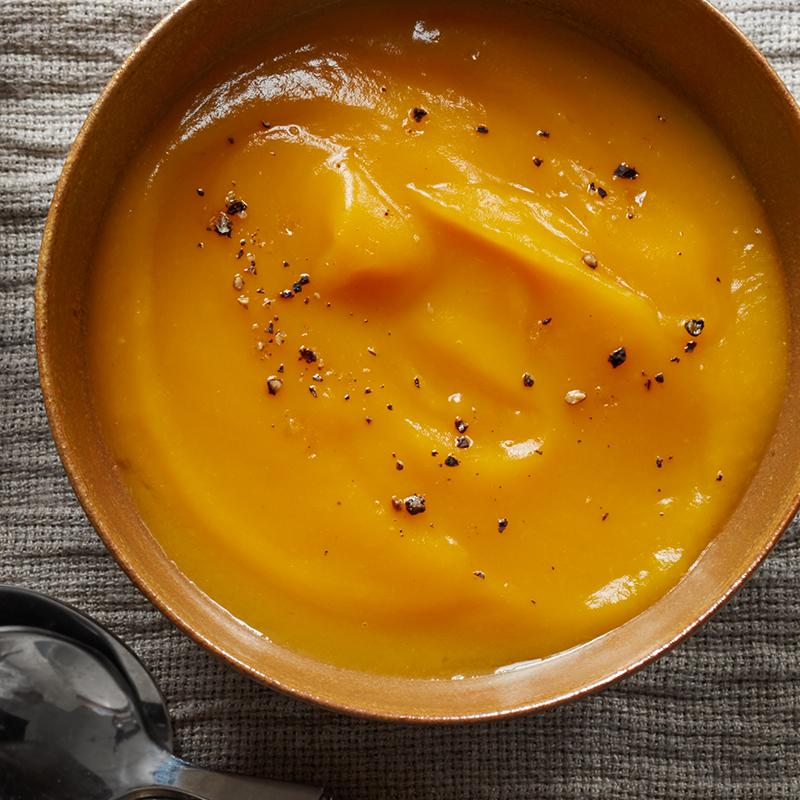
\includegraphics[width=0.9\linewidth]{/home/tim/Documents/projects/recipes/img/squash_bisque.jpg}\\
\end{minipage}\vspace{3mm}
\textbf{Directions}:
\vspace{-3mm}\begin{enumerate}\setlength\itemsep{-1mm}
\item Heat butter in soup pot over medium heat. Add onion and salt; cook, stirring occasionally, until onion is softened (5-7 minutes).
\item Add garlic, nutmeg and cayenne; stir and cook 1 minute. Add squash and broth; bring to a boil over high heat.
\item Reduce heat to low and simmer, uncovered, until squash is soft, about 30 minutes; stir in yogurt and sugar.
\item Remove from heat and puree soup in pot. Serve garnished with fresh sage and black pepper.
\end{enumerate}
\end{minipage}\vspace{8mm}
\noindent\begin{minipage}[t]{\linewidth}%
{\Large\textbf{Chicken Taco Stew}} \label{chicken-taco-stew}\hfill\textit{Sue Dunn}\\
\noindent\begin{minipage}[t]{0.78\linewidth}%
\textbf{Ingredients}:\vspace{-3mm}
\begin{multicols}{2}
\begin{itemize}\setlength\itemsep{-1mm}
\item 1 sweet onion, chopped
\item 1 can cannellini beans, drained and rinsed
\item 1 can black beans, drained and rinsed
\item 3 (10 oz) cans of diced tomatoes with green chillies
\item 1 packet taco seasoning
\item 1 can sweet corn, drained
\item 3 skinless boneless chicken breasts cut lengthwise in half
\item 3 avocados, chopped
\end{itemize}
\end{multicols}
\end{minipage}
\noindent\begin{minipage}[t]{0.18\linewidth}
\centering \strut\vspace*{-\baselineskip}\newline
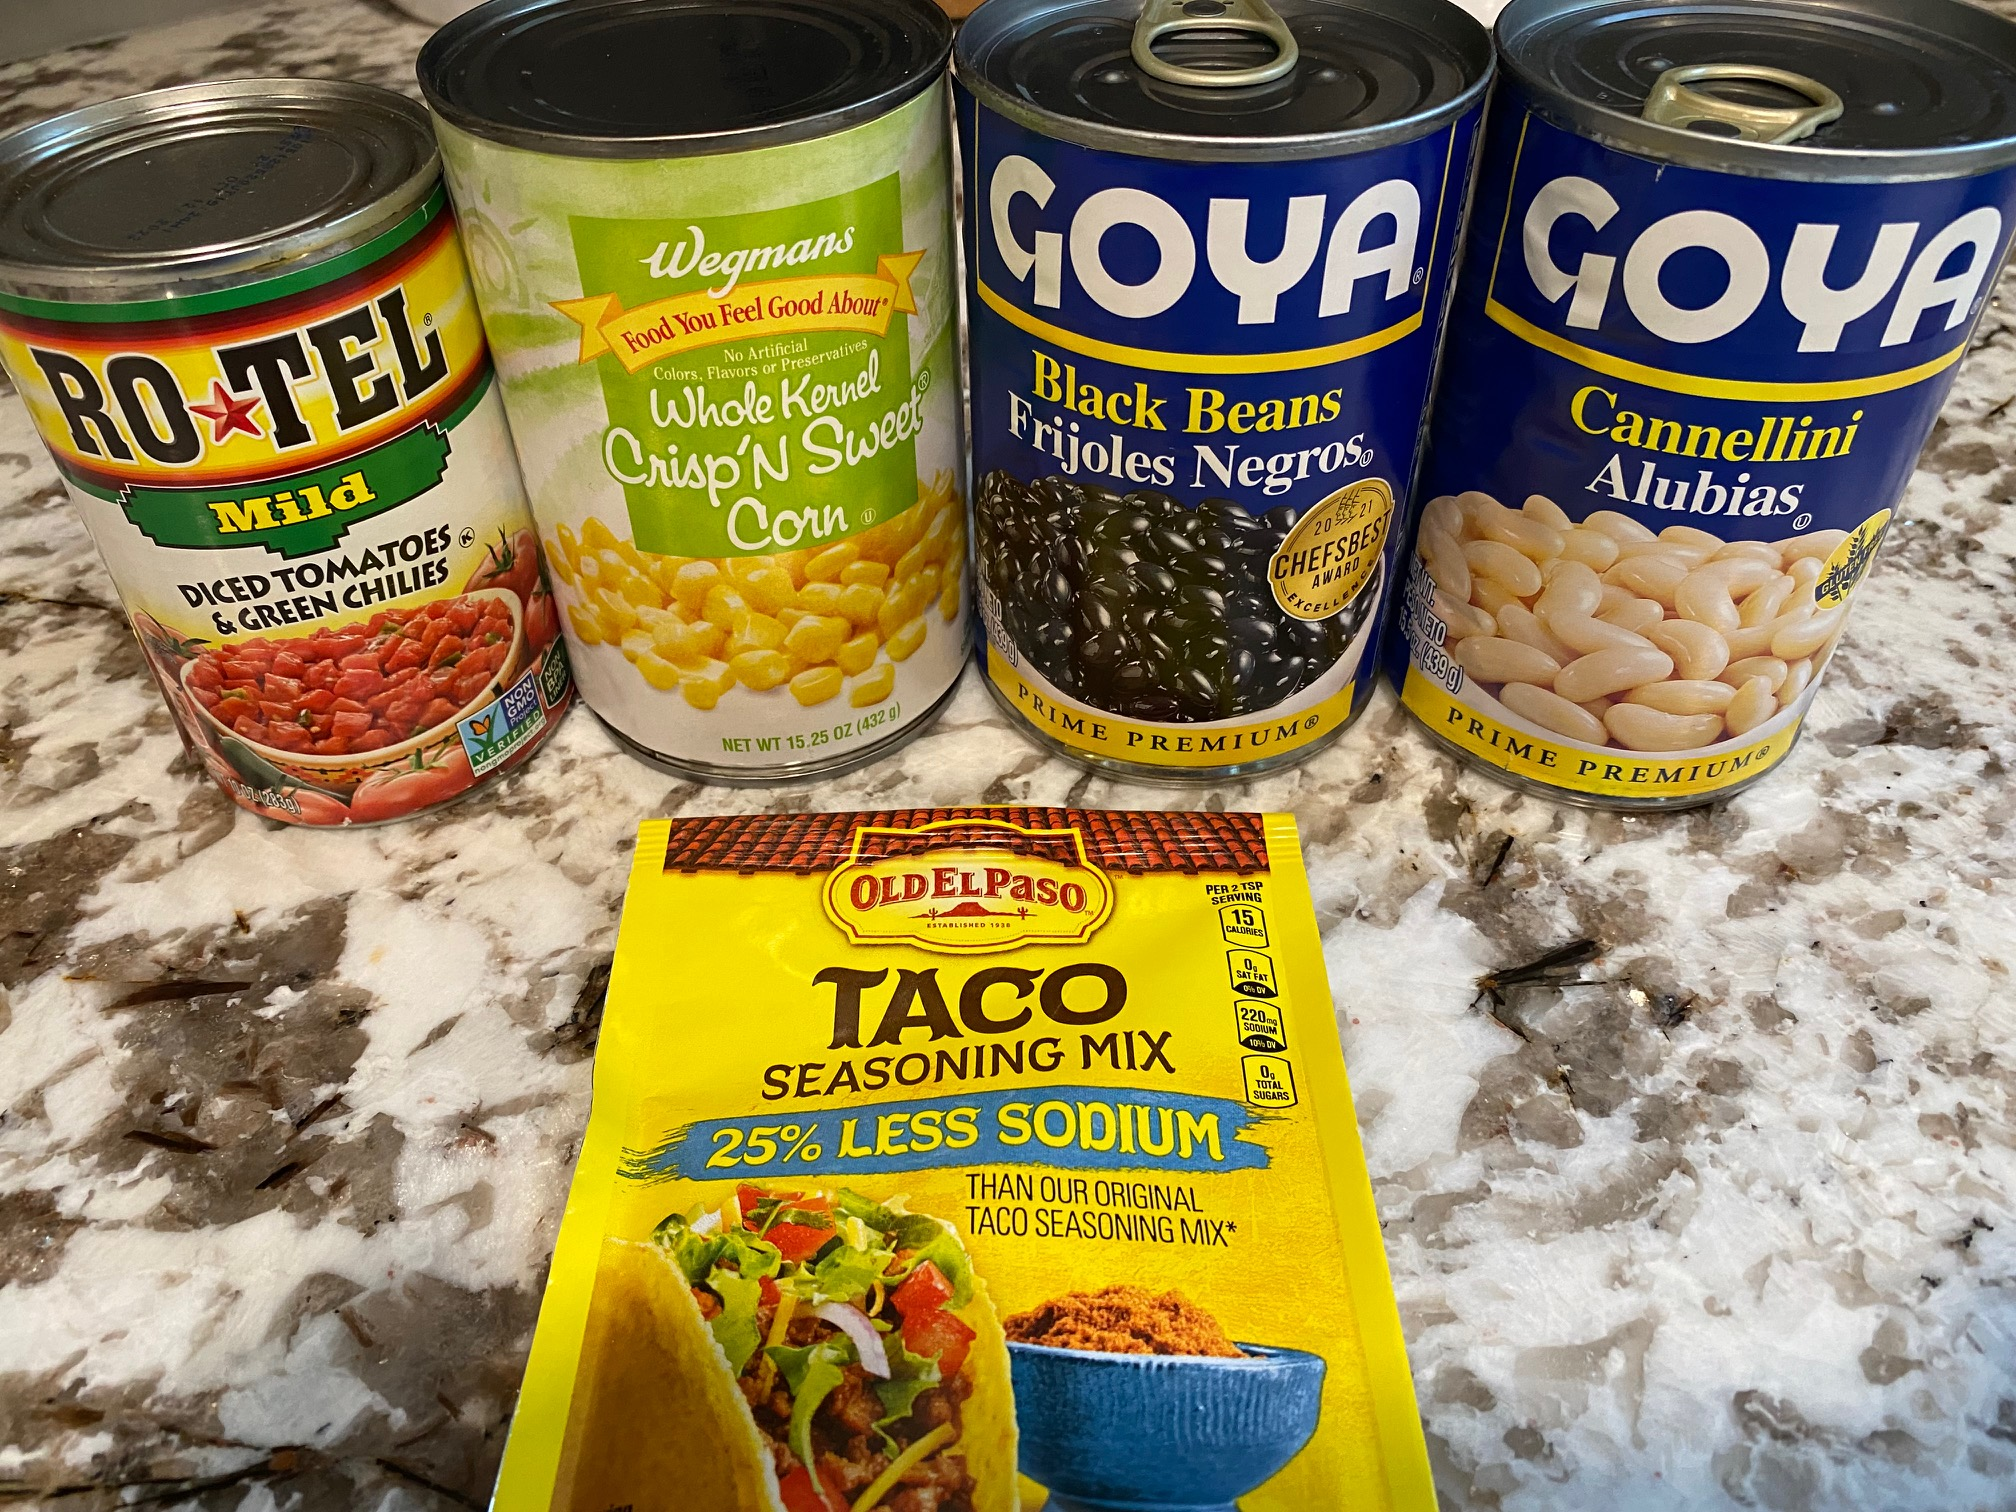
\includegraphics[width=0.9\linewidth]{/home/tim/Documents/projects/recipes/img/taco_stew.jpg}\\
\end{minipage}\vspace{3mm}
\textbf{Directions}:
\vspace{-3mm}\begin{enumerate}\setlength\itemsep{-1mm}
\item Mix everything together in a slow cooker except chicken. Lay chicken on top and cover. Cook on low for 6-8 hours or on high for 4 hours.
\item 30 minutes before serving, remove chicken and shred. Return shredded chicken to slow cooker and stir in. This is good eaten with cheese, sour cream, or tortilla chips and of course fresh avacados on top.
\end{enumerate}
\end{minipage}\vspace{8mm}
\noindent\begin{minipage}[t]{\linewidth}%
{\Large\textbf{Corn Chowder}} \label{corn-chowder}\hfill\textit{Sue Dunn}\\
\textbf{Yield:} \textit{18 cups}\\
\noindent\begin{minipage}[t]{0.78\linewidth}%
\textbf{Ingredients}:\vspace{-3mm}
\begin{multicols}{2}
\begin{itemize}\setlength\itemsep{-1mm}
\item 1 pkg (4 oz) Italian Classics Diced Pancetta
\item 1 cup chopped onion
\item 1 cup diced celery
\item 3 cloves garlic, minced
\item 6 Tbsp salted butter
\item 1/2 cup all-purpose flour
\item 2 (32 oz) cartons chicken stock
\item 8 ears fresh corn, shucked, kernels removed
\item 1 red bell pepper, diced
\item 1 large russet potato, peeled, diced
\item 1 Tbsp chopped thyme
\item 1 1/4 tsp sea salt
\item black pepper
\item 2 (8 oz) cartons light cream
\item 1 tsp tabasco sauce
\item 1 tsp Old Bay seasoning
\end{itemize}
\end{multicols}
\end{minipage}
\noindent\begin{minipage}[t]{0.18\linewidth}
\centering \strut\vspace*{-\baselineskip}\newline
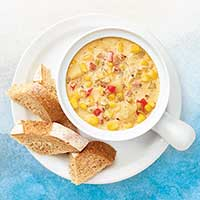
\includegraphics[width=0.9\linewidth]{/home/tim/Documents/projects/recipes/img/corn_chowder.jpg}\\
\end{minipage}\vspace{3mm}
\textbf{Directions}:
\vspace{-3mm}\begin{enumerate}\setlength\itemsep{-1mm}
\item Add pancetta to pot on medium. Cook 2-3 min, until crispy. Add onion, celery, and garlic; stir. Cook about 4 min, until soft but not browned.
\item Add butter; stir until melted and it begins to bubble. Add flour, stirring until completely blended. Cook, stirring and scraping bottom of pot every 30 seconds, about 3 min.
\item Whisk in chicken stock. Add corn; whisk. Add peppers, potato, and thyme; season to taste with sea salt and freshly ground pepper. Increase heat to medium-high. Cook, stirring occasionally, about 10 min until it comes to a boil.
\item Reduce heat to medium. Simmer 10-15 min until potato is tender. Add cream gradually; stir. Return to simmer, about 2-3 min. Season with Tabasco and Old Bay.
\end{enumerate}
\end{minipage}\vspace{8mm}
\noindent\begin{minipage}[t]{\linewidth}%
{\Large\textbf{Egg Drop Soup}} \label{egg-drop-soup}\hfill\textit{Carolyn Benjamin}\\
\noindent\begin{minipage}[t]{0.78\linewidth}%
\textbf{Ingredients}:\vspace{-3mm}
\begin{multicols}{2}
\begin{itemize}\setlength\itemsep{-1mm}
\item 3 Cups Chicken stock (college inn)
\item 1 Egg (Beaten)
\item 1 Scallion (Chopped)
\item 1 Tbsp cornstarch
\item 1 Tbsp Water
\end{itemize}
\end{multicols}
\end{minipage}
\noindent\begin{minipage}[t]{0.18\linewidth}
\centering \strut\vspace*{-\baselineskip}\newline
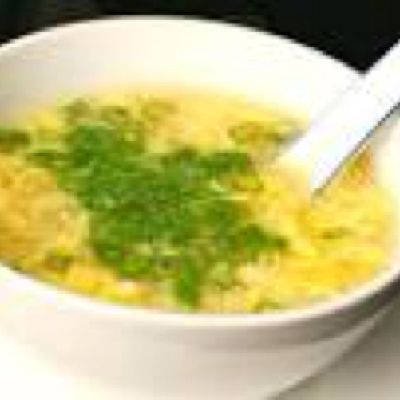
\includegraphics[width=0.9\linewidth]{/home/tim/Documents/projects/recipes/img/FD6D1C2E-051B-4FA3-98AC-2E4FF82BBA09.jpg}\\
\end{minipage}\vspace{3mm}
\textbf{Directions}:
\vspace{-3mm}\begin{enumerate}\setlength\itemsep{-1mm}
\item Put stock on high heat.
\item While boiling, stir in cornstarch until stock thickens and becomes clear.
\item Slowly pour in egg and stir once gently.
\item Turn off heat. Pour in bowls and top with chopped scallions.
\end{enumerate}
\end{minipage}\vspace{8mm}
\noindent\begin{minipage}[t]{\linewidth}%
{\Large\textbf{Potato Leek Soup}} \label{potato-leek-soup}\hfill\textit{Sue Dunn}\\
\textbf{Yield:} \textit{Serves 8-10}\\
\noindent\begin{minipage}[t]{0.78\linewidth}%
\textbf{Ingredients}:\vspace{-3mm}
\begin{multicols}{2}
\begin{itemize}\setlength\itemsep{-1mm}
\item 1/4 cup unsalted butter
\item 2 lb leeks, white portions only, trimmed, carefully washed and thinly sliced
\item 6 cups chicken/vegetable stock
\item 2 lb baking potatoes, peeled, quartered lengthwise and thinly sliced
\item salt and white pepper
\item 2 Tbsp finely chopped fresh chives
\end{itemize}
\end{multicols}
\end{minipage}
\noindent\begin{minipage}[t]{0.18\linewidth}
\centering \strut\vspace*{-\baselineskip}\newline
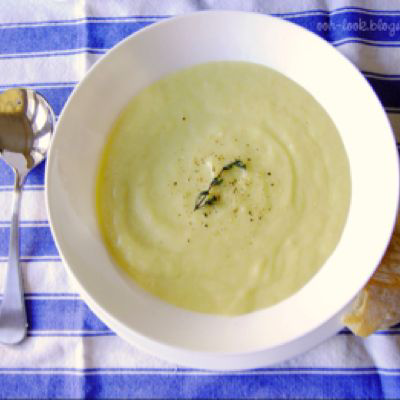
\includegraphics[width=0.9\linewidth]{/home/tim/Documents/projects/recipes/img/511D727A-8A5C-4025-B07A-B7168B6B53CF.jpg}\\
\end{minipage}\vspace{3mm}
\textbf{Directions}:
\vspace{-3mm}\begin{enumerate}\setlength\itemsep{-1mm}
\item In a large saucepan, melt the butter over medium heat. Add the leeks and saute just until they begin to soften, 3-5 minutes. Add the stock and potatoes, bring to a boil, reduce heat to low, cover, and simmer until the potatoes are very tender, about 20 minutes. 
\item Use handheld blender to puree the soup. Season to taste with salt and white pepper. Ladle into warmed bowls and garnish with the chives.
\end{enumerate}
\end{minipage}\vspace{8mm}
\noindent\begin{minipage}[t]{\linewidth}%
{\Large\textbf{Spicy White Turkey Chili Soup}} \label{spicy-white-turkey-chili-soup}\hfill\textit{Sue Dunn}\\
\textbf{Yield:} \textit{15 cups}\\
\noindent\begin{minipage}[t]{0.78\linewidth}%
\textbf{Ingredients}:\vspace{-3mm}
\begin{multicols}{2}
\begin{itemize}\setlength\itemsep{-1mm}
\item 2 Tbsp butter
\item 3 Tbsp olive oil
\item 1 1/2 cups diced celery and onions
\item 3/4 cup all-purpose flour
\item 3 Tbsp chili powder
\item 1 tsp cumin
\item 1/8 tsp cayenne pepper
\item 2 (32 oz) cartons chicken culinary stock
\item 1 red bell pepper, diced
\item 2 (15.5 oz) cans cannellini beans
\item 1 green bell pepper, diced
\item 1 cup (6 oz) cooked turkey, diced
\item 1/4 cup heavy cream
\item salt and pepper to taste
\end{itemize}
\end{multicols}
\end{minipage}
\noindent\begin{minipage}[t]{0.18\linewidth}
\centering \strut\vspace*{-\baselineskip}\newline

\includegraphics[width=0.9\linewidth]{/home/tim/Documents/projects/recipes/img/none.jpg}\\
\end{minipage}\vspace{3mm}
\textbf{Directions}:
\vspace{-3mm}\begin{enumerate}\setlength\itemsep{-1mm}
\item Melt butter and olive oil in large stockpot on medium, until oil/butter mixture faintly smokes. Add celery and onions. Cool, stirring occasionally for 4-5 minutes, until translucent but not brown. Stir in flour, chili powder, cumin and cayenne. Cook 1 more minute, stirring continuously.
\item Add stock. Bring to a simmer; simmer 10 minutes. Add cannellini beans, peppers, turkey and heavy cream. Season to taste with salt and pepper. Simmer 2-3 minutes until heated through. Ladle into warmed bowls.
\end{enumerate}
\end{minipage}\vspace{8mm}

{\newpage \LARGE \textbf{Sides}} \label{sides}\\
\noindent\begin{minipage}[t]{\linewidth}%
{\Large\textbf{Blueberry Muffins}} \label{blueberry-muffins}\hfill\textit{}\\
\noindent\begin{minipage}[t]{0.78\linewidth}%
\textbf{Ingredients}:\vspace{-3mm}
\begin{multicols}{2}
\begin{itemize}\setlength\itemsep{-1mm}
\item 3 cups flour
\item 1 cup sugar
\item 4 tsp baking powder
\item 1 tsp salt
\item 2 eggs, lightly beaten
\item 1/2 cup oil
\item 1 cup milk
\item 1 1/2 cups blueberries
\end{itemize}
\end{multicols}
\end{minipage}
\noindent\begin{minipage}[t]{0.18\linewidth}
\centering \strut\vspace*{-\baselineskip}\newline
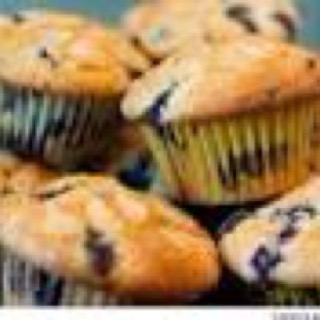
\includegraphics[width=0.9\linewidth]{/home/tim/Documents/projects/recipes/img/C369CD3B-128B-453F-8459-2D584B138E81.jpg}\\
\end{minipage}\vspace{3mm}
\textbf{Directions}:
\vspace{-3mm}\begin{enumerate}\setlength\itemsep{-1mm}
\item Preheat oven to 400F.
\item Mix together flour, sugar, baking powder and salt. Combine eggs and milk and stir into dry ingredients until moistened.
\item Add and stir the berries through the mixture. Spoon into muffin tins about half full.
\item Bake for 20 minutes.
\end{enumerate}
\end{minipage}\vspace{8mm}
\noindent\begin{minipage}[t]{\linewidth}%
{\Large\textbf{Sweet Potatoes Mashed}} \label{sweet-potatoes-mashed}\hfill\textit{}\\
\noindent\begin{minipage}[t]{0.78\linewidth}%
\textbf{Ingredients}:\vspace{-3mm}
\begin{multicols}{2}
\begin{itemize}\setlength\itemsep{-1mm}
\item 5 Medium (4 lb) Sweet potatoes (yams), peeled, 1 in. dice (10 cups)
\item 1 1/4 Cups Whole milk
\item 1 Stick (1/2 cup) Wegmans' unsalted butter
\item 1/3 Cup Brown Sugar
\item 1 1/2 tsp McCormick Ground Cinnamon
\item Salt and pepper to taste
\item You'll need: potato masher
\end{itemize}
\end{multicols}
\end{minipage}
\noindent\begin{minipage}[t]{0.18\linewidth}
\centering \strut\vspace*{-\baselineskip}\newline
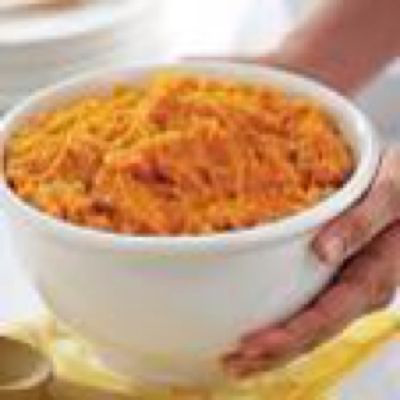
\includegraphics[width=0.9\linewidth]{/home/tim/Documents/projects/recipes/img/2E22A92B-794C-45CB-9160-95C5F86B3074.jpg}\\
\end{minipage}\vspace{3mm}
\textbf{Directions}:
\vspace{-3mm}\begin{enumerate}\setlength\itemsep{-1mm}
\item Place potatoes in stock pot; cover with cold water. Bring to boil on high; reduce heat to medium. Cover and simmer potatoes about 15 mins, until tender when pierced with knife tip. Drain; return to stockpot. Heat on low 3-5 mins, tossing gently, to remove excess moisture.
\item Combine potatoes, milk, butter, brown sugar, and cinnamon in stockpot. Mash with with handheld potato masher. Season to taste with salt and pepper. 
\end{enumerate}
\end{minipage}\vspace{8mm}

{\newpage \LARGE \textbf{Breakfasts}} \label{breakfasts}\\
\noindent\begin{minipage}[t]{\linewidth}%
{\Large\textbf{Ham and Broccoli Casserole}} \label{ham-and-broccoli-casserole}\hfill\textit{}\\
\textbf{Yield:} \textit{Serves 10-12}\\
\noindent\begin{minipage}[t]{0.78\linewidth}%
\textbf{Ingredients}:\vspace{-3mm}
\begin{multicols}{2}
\begin{itemize}\setlength\itemsep{-1mm}
\item 12 small slices white bread, crusts removed, torn into pieces
\item 3 cups cooked, cubed ham
\item 3 cups chopped frozen broccoli, thawed
\item 8 oz shredded sharp cheddar cheese
\item 1/2 cup milk
\item 6 eggs, beaten
\item 1 1/4 tsp salt
\item 1 tsp dry mustard
\item 2 Tbsp melted butter
\end{itemize}
\end{multicols}
\end{minipage}
\noindent\begin{minipage}[t]{0.18\linewidth}
\centering \strut\vspace*{-\baselineskip}\newline
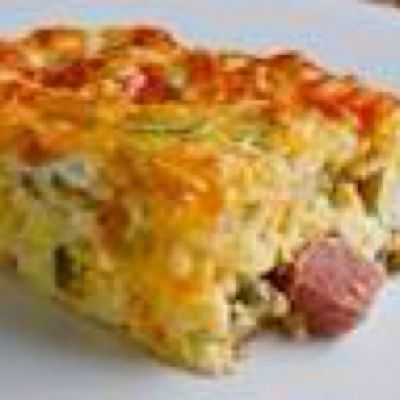
\includegraphics[width=0.9\linewidth]{/home/tim/Documents/projects/recipes/img/D08AE61F-C771-49C4-8DD1-111FCF4EA38E.jpg}\\
\end{minipage}\vspace{3mm}
\textbf{Directions}:
\vspace{-3mm}\begin{enumerate}\setlength\itemsep{-1mm}
\item In a 9x13x2 inch baking dish, put enough of the bread pieces into the bottom of the pan to make a thin layer. Make a layer of ham, broccoli, and cheese. Whisk together milk, eggs, salt, and dry mustard. Pour over top. Toss remaining bread with butter; sprinkle over the top of the casserole. Bake at 325F for 45 minutes. Let cool for about 20 minutes.
\end{enumerate}
\end{minipage}\vspace{8mm}
\noindent\begin{minipage}[t]{\linewidth}%
{\Large\textbf{Pancakes}} \label{pancakes}\hfill\textit{Carolyn Benjamin}\\
\noindent\begin{minipage}[t]{0.78\linewidth}%
\textbf{Ingredients}:\vspace{-3mm}
\begin{multicols}{2}
\begin{itemize}\setlength\itemsep{-1mm}
\item 1 1/2 cups all-purpose flour
\item 3 1/2 tsp baking powder
\item 1 tsp salt
\item 1 Tbsp white sugar
\item 1 1/4 cups milk
\item 1 egg
\item 3 Tbsp butter, melted
\end{itemize}
\end{multicols}
\end{minipage}
\noindent\begin{minipage}[t]{0.18\linewidth}
\centering \strut\vspace*{-\baselineskip}\newline
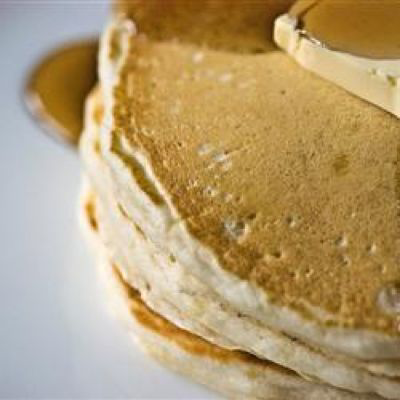
\includegraphics[width=0.9\linewidth]{/home/tim/Documents/projects/recipes/img/8345AC64-F6A9-48FE-ACE0-4D19E230A1B3.jpg}\\
\end{minipage}\vspace{3mm}
\textbf{Directions}:
\vspace{-3mm}\begin{enumerate}\setlength\itemsep{-1mm}
\item In a large bowl, sift together the flour, baking powder, salt and sugar. Make a well in the center and pour in the milk, egg and melted butter; mix until smooth.
\item Heat a lightly oiled griddle or frying pan over medium high heat. Pour or scoop the batter onto the griddle, using approximately 1/4 cup for each pancake. Brown on both sides and serve hot.
\end{enumerate}
\end{minipage}\vspace{8mm}
\noindent\begin{minipage}[t]{\linewidth}%
{\Large\textbf{Pumpkin Waffles}} \label{pumpkin-waffles}\hfill\textit{Aunt Carolyn Benjamin}\\
\textbf{Yield:} \textit{8 waffles}\\
\noindent\begin{minipage}[t]{0.78\linewidth}%
\textbf{Ingredients}:\vspace{-3mm}
\begin{multicols}{2}
\begin{itemize}\setlength\itemsep{-1mm}
\item 1 cup flour
\item 2 tsp baking powder
\item 3/4 tsp ground cinnamon
\item 1/8 tsp salt
\item 1/8 tsp ground cloves
\item 1 cup low fat milk
\item 1/2 cup pumpkin puree
\item 1/4 cup packed dark brown sugar
\item 1 Tbsp vegetable oil
\item 1 large egg, slightly beaten
\end{itemize}
\end{multicols}
\end{minipage}
\noindent\begin{minipage}[t]{0.18\linewidth}
\centering \strut\vspace*{-\baselineskip}\newline
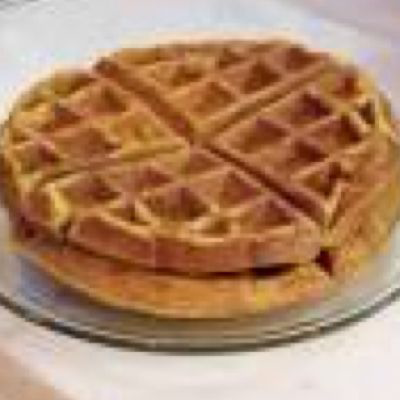
\includegraphics[width=0.9\linewidth]{/home/tim/Documents/projects/recipes/img/6F6656B5-56C4-49D2-A435-402CEA169684.jpg}\\
\end{minipage}\vspace{3mm}
\textbf{Directions}:
\vspace{-3mm}\begin{enumerate}\setlength\itemsep{-1mm}
\item Combine flour and next four ingredients (through cloves) in a large bowl. Make a well in the center of the mixture.
\item Combine milk and next four ingredients (through egg) in a bowl and add flour mixture. Stir until moist.
\item Coat waffle iron with cooking spray (if necessary). Spoon about 1/4 cup batter per waffle into hot waffle iron, spreading batter to edges
\end{enumerate}
\end{minipage}\vspace{8mm}

{\newpage \LARGE \textbf{Dips}} \label{dips}\\

{\newpage \LARGE \textbf{Seafood}} \label{seafood}\\
\noindent\begin{minipage}[t]{\linewidth}%
{\Large\textbf{Bourbon Bacon Scallops}} \label{bourbon-bacon-scallops}\hfill\textit{}\\
\noindent\begin{minipage}[t]{0.78\linewidth}%
\textbf{Ingredients}:\vspace{-3mm}
\begin{multicols}{2}
\begin{itemize}\setlength\itemsep{-1mm}
\item 6 slices bacon (4-5 oz)
\item 3 Tbsp minced scallions (green onions)
\item 2 Tbsp bourbon
\item 2 Tbsp maple syrup
\item 1 Tbsp soy sauce
\item 1 Tbsp Dijon mustard
\item 1/4 tsp fresh ground black pepper or 1/4 teaspoon fresh ground tricolor pepper 24 large sea scallops cooking spray (about 1 1/2 pounds)
\item 24 Large sea scallops (about 1 1/2 pounds)
\item cooking spray
\item 4 metal skewers or 4 water-soaked bamboo skewers (12 inch)
\end{itemize}
\end{multicols}
\end{minipage}
\noindent\begin{minipage}[t]{0.18\linewidth}
\centering \strut\vspace*{-\baselineskip}\newline
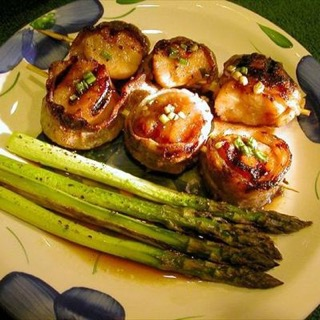
\includegraphics[width=0.9\linewidth]{/home/tim/Documents/projects/recipes/img/7BA081E5-C2CE-4A48-A94B-73154236B71B.jpg}\\
\end{minipage}\vspace{3mm}
\textbf{Directions}:
\vspace{-3mm}\begin{enumerate}\setlength\itemsep{-1mm}
\item 1 Heat a skillet over high temperature and saute the bacon for 4-5 minutes, until limp and partially browned; remove from skillet, drain, and set aside to cool. 
\item 2 In a bowl, combine the green onions, bourbon, maple syrup, soy sauce, mustard, and pepper, and stir well; remove about 2 tablespoons of marinade to another container and set aside. 
\item 3 Add the sea scallops to the marinade in the bowl and toss gently to coat. 
\item 4 Cover and place in refrigerator to marinate for 1 hour, stirring occasionally. 
\item 5 Preheat your oven broiler; pan spray a broiler pan. 
\item 6 Cut the partially cooked bacon strips into 4 sections apiece. 
\item 7 Remove the scallops from the marinade (reserve marinade) and wrap a piece of cut bacon around each scallop - if the scallops are very large, they might only reach halfway around. 
\item 8 Thread the wrapped scallops onto the skewers (going through each end of bacon strips if they only reach halfway around), making sure to leave space between each scallop so that the bacon will cook well. 
\item 9 Place the completed skewers on the pan-sprayed boiler pan and broil for 8 minutes or until the bacon is crisp and the scallops are opaque, occasionally basting with the marinade used with the scallops (how long they need to cook depends on the size of the scallops). 
\item 10 Remove skewers from broiler, place them on a serving platter, and brush or drizzle with the reserved marinade (that which was not combined with the scallops in the refrigerator). 
\item 11 Note: these can also be cooked on the grill if you watch them carefully so that the scallops do not overcook.
\end{enumerate}
\end{minipage}\vspace{8mm}
\noindent\begin{minipage}[t]{\linewidth}%
{\Large\textbf{Coconut Shrimp}} \label{coconut-shrimp}\hfill\textit{Sue Dunn}\\
\noindent\begin{minipage}[t]{0.78\linewidth}%
\textbf{Ingredients}:\vspace{-3mm}
\begin{multicols}{2}
\begin{itemize}\setlength\itemsep{-1mm}
\item 2 large egg whites
\item 3/4 cup all purpose flour
\item 6 oz beer
\item 1 1/2 tsp baking powder
\item 1/4 tsp table salt
\item 2 cups sweetened coconut flakes
\item 24 large uncooked shrimp, peeled and deveined (leave tails on)
\end{itemize}
\end{multicols}
\end{minipage}
\noindent\begin{minipage}[t]{0.18\linewidth}
\centering \strut\vspace*{-\baselineskip}\newline
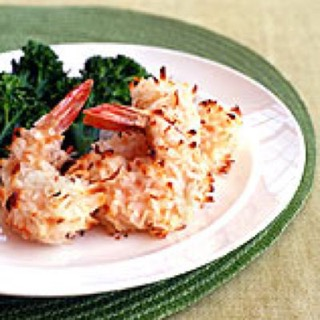
\includegraphics[width=0.9\linewidth]{/home/tim/Documents/projects/recipes/img/623F2F31-CC8C-40B2-9D59-DED8927C64FD.jpg}\\
\end{minipage}\vspace{3mm}
\textbf{Directions}:
\vspace{-3mm}\begin{enumerate}\setlength\itemsep{-1mm}
\item Preheat oven to 450F. Coat a large baking sheet with cooking spray.
\item In a medium bowl, whisk together egg whites, 1/2 cup of flour, beer, baking powder and salt. Place remaining 1/4 cup of flour and coconut in two separate shallow bowls.
\item Holding shrimp by their tails, dredge each shrimp in flour and shake off any excess. Dip flour-coated shrimp into egg batter and allow excess to drip off. Roll shrimp in coconut and turn to coat both sides (press coconut onto shrimp to make it stick).
\item Transfer shrimp to prepared baking sheet and spray surface of shrimp with cooking spray.
\item Bake until coconut is golden brown and shrimp are bright pink and cooked through (10-12 minutes).
\end{enumerate}
\end{minipage}\vspace{8mm}
\noindent\begin{minipage}[t]{\linewidth}%
{\Large\textbf{Crab Casserole}} \label{crab-casserole}\hfill\textit{Mom}\\
\noindent\begin{minipage}[t]{0.78\linewidth}%
\textbf{Ingredients}:\vspace{-3mm}
\begin{multicols}{2}
\begin{itemize}\setlength\itemsep{-1mm}
\item 1 Tbsp margerine
\item 2 scallion, chopped
\item 1 tsp cornstarch
\item 1/2 cup half-and-half cream
\item 2 tsp lemon juice
\item 1/8 tsp salt
\item 1/8 tsp pepper
\item 2/3 cup cooked crabmeat
\item 4 mushrooms (Sliced)
\item 2 Tbsp dry bread crumbs
\item 1 1/3 Tbsp grated Parmesan cheese
\item 1 Tbsp melted margerine
\end{itemize}
\end{multicols}
\end{minipage}
\noindent\begin{minipage}[t]{0.18\linewidth}
\centering \strut\vspace*{-\baselineskip}\newline
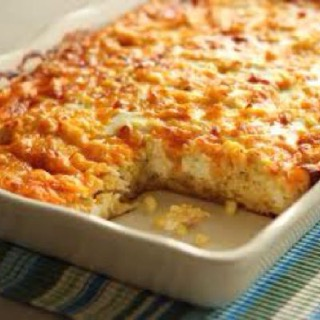
\includegraphics[width=0.9\linewidth]{/home/tim/Documents/projects/recipes/img/AE88C0C2-4A05-4022-A9F4-C438F2053528.jpg}\\
\end{minipage}\vspace{3mm}
\textbf{Directions}:
\vspace{-3mm}\begin{enumerate}\setlength\itemsep{-1mm}
\item Put margarine and onion in a bowl. Microwave uncovered until crisp.
\item Mix in cornstarch, stir in half and half, lemon juice, salt, and pepper. Microwave uncovered for one minute. Stir, and microwave for another minute. Stir in the crab and mushroom.
\item Mix topping, sprinkle on top, cover loosely, and microwave until hot.
\end{enumerate}
\end{minipage}\vspace{8mm}
\noindent\begin{minipage}[t]{\linewidth}%
{\Large\textbf{Honey Balsamic Salmon}} \label{honey-balsamic-salmon}\hfill\textit{}\\
\noindent\begin{minipage}[t]{0.78\linewidth}%
\textbf{Ingredients}:\vspace{-3mm}
\begin{multicols}{2}
\begin{itemize}\setlength\itemsep{-1mm}
\item 1/4 tsp olive oil
\item 1/2 cup leek(s), julienne-cut (about 1 small)
\item 1 1/2 lb salmon fillets, with or without skin, four 6-oz. pieces
\item 1/2 tsp table salt, divided
\item 1/4 tsp black pepper, divided
\item 1/2 cup balsamic vinegar
\item 1 Tbsp honey
\end{itemize}
\end{multicols}
\end{minipage}
\noindent\begin{minipage}[t]{0.18\linewidth}
\centering \strut\vspace*{-\baselineskip}\newline
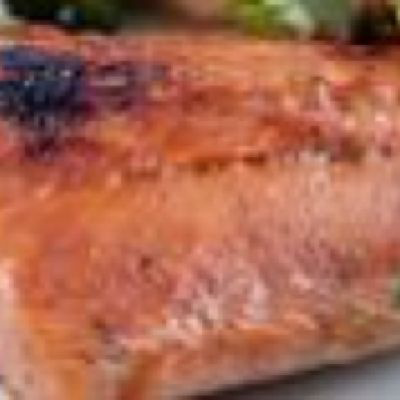
\includegraphics[width=0.9\linewidth]{/home/tim/Documents/projects/recipes/img/53AC6E19-DE06-4A08-87E0-2EBE21E19FB6.jpg}\\
\end{minipage}\vspace{3mm}
\textbf{Directions}:
\vspace{-3mm}\begin{enumerate}\setlength\itemsep{-1mm}
\item Coat a large nonstick skillet with cooking spray; add oil. Place over medium-high heat; add leaks and saute 3 to 4 minutes or until soft. Remove from pan and set aside.
\item Sprinkle fish with 1/4 tsp salt and 1/8 tsp pepper. Add fish to pan; cook 3 to 4 minutes on each side or until lightly browned and fish flakes easily when tested with a fork. Remove from pan; set aside, and keep warm.
\item Add vinegar, honey, 1/4 tsp salt, and 1/8 tsp pepper to pan. Cook over medium-high heat 3-4 minutes or until reduced by half. Divide leaks evenly over fish; drizzle with sauce. 
\end{enumerate}
\end{minipage}\vspace{8mm}
\noindent\begin{minipage}[t]{\linewidth}%
{\Large\textbf{Pan-Seared Scallops}} \label{pan-seared-scallops}\hfill\textit{}\\
\textbf{Yield:} \textit{4 servings}\\
\noindent\begin{minipage}[t]{0.78\linewidth}%
\textbf{Ingredients}:\vspace{-3mm}
\begin{multicols}{2}
\begin{itemize}\setlength\itemsep{-1mm}
\item 1 lb fresh sea scallops
\item salt and pepper
\item pan searing flour
\item 1 Tbsp olive oil
\item 2 Tbsp shallot-thyme finishing butter
\end{itemize}
\end{multicols}
\end{minipage}
\noindent\begin{minipage}[t]{0.18\linewidth}
\centering \strut\vspace*{-\baselineskip}\newline
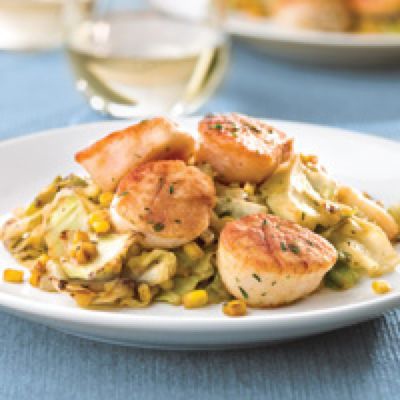
\includegraphics[width=0.9\linewidth]{/home/tim/Documents/projects/recipes/img/7A83B49C-ECC8-4B52-B5AD-C50C8B011C37.jpg}\\
\end{minipage}\vspace{3mm}
\textbf{Directions}:
\vspace{-3mm}\begin{enumerate}\setlength\itemsep{-1mm}
\item Season scallops with salt and pepper; dust with pan-searing flour. Heat olive oil in pan on medium-high; add scallops. Sear until golden brown (2-3 minutes). Turn scallops.
\item Reduce heat to medium-low. Cook for 2-3 minutes, until internal temperature reaches 120F.
\item Add butter and baste scallops for 1-2 minutes until internal temp reaches 130F. Let scallops rest for 2 minutes.
\end{enumerate}
\end{minipage}\vspace{8mm}

{\newpage \LARGE \textbf{Steak}} \label{steak}\\
\noindent\begin{minipage}[t]{\linewidth}%
{\Large\textbf{Steak Teriyaki Marinade}} \label{steak-teriyaki-marinade}\hfill\textit{Aunt Nancy Feth}\\
\noindent\begin{minipage}[t]{0.78\linewidth}%
\textbf{Ingredients}:\vspace{-3mm}
\begin{multicols}{2}
\begin{itemize}\setlength\itemsep{-1mm}
\item 3/4 cup soy sauce
\item 1/4 cup water or wine
\item 1 tsp garlic powder
\item 2 tsp sugar
\item 1/2 tsp ginger
\end{itemize}
\end{multicols}
\end{minipage}
\noindent\begin{minipage}[t]{0.18\linewidth}
\centering \strut\vspace*{-\baselineskip}\newline
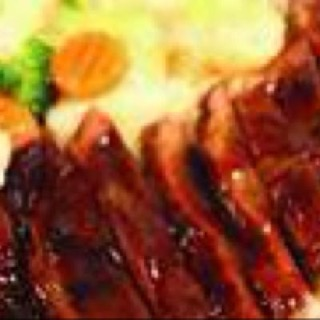
\includegraphics[width=0.9\linewidth]{/home/tim/Documents/projects/recipes/img/041AD6E5-03E7-484A-B58E-E8678B694B63.jpg}\\
\end{minipage}\vspace{3mm}
\textbf{Directions}:
\vspace{-3mm}\begin{enumerate}\setlength\itemsep{-1mm}
\item Mix all together and pour over meat to be marinated. Double recipe to desired quantity to cover meat.
\end{enumerate}
\end{minipage}\vspace{8mm}

{\newpage \LARGE \textbf{Pork}} \label{pork}\\
\noindent\begin{minipage}[t]{\linewidth}%
{\Large\textbf{Barbecue Sauce}} \label{barbecue-sauce}\hfill\textit{Uncle Tim Dunn}\\
\textbf{Yield:} \textit{}\\
\noindent\begin{minipage}[t]{0.78\linewidth}%
\textbf{Ingredients}:\vspace{-3mm}
\begin{multicols}{2}
\begin{itemize}\setlength\itemsep{-1mm}
\item 1 cup water
\item 3 cups apple cider vinegar
\item 4 cups brown sugar
\item 3 Tbsp onion powder
\item 1 Tbsp paprika
\item 1 Tbsp black pepper
\item 1/2 Tbsp garlic powder
\item 1 cup ketchup
\item 2 cup BBQ sauce
\item 2 Tbsp Worchestershire sauce
\end{itemize}
\end{multicols}
\end{minipage}
\noindent\begin{minipage}[t]{0.18\linewidth}
\centering \strut\vspace*{-\baselineskip}\newline

\includegraphics[width=0.9\linewidth]{/home/tim/Documents/projects/recipes/img/none.jpg}\\
\end{minipage}\vspace{3mm}
\textbf{Directions}:
\vspace{-3mm}\begin{enumerate}\setlength\itemsep{-1mm}
\item Mix ingredients thoroughly.
\end{enumerate}
\end{minipage}\vspace{8mm}
\noindent\begin{minipage}[t]{\linewidth}%
{\Large\textbf{Rib Sauce}} \label{rib-sauce}\hfill\textit{Grandma Claire Dunn}\\
\noindent\begin{minipage}[t]{0.78\linewidth}%
\textbf{Ingredients}:\vspace{-3mm}
\begin{multicols}{2}
\begin{itemize}\setlength\itemsep{-1mm}
\item 1 cup OJ
\item 1 lemon
\item 1 cup brown sugar
\item 3/4 cup pancake syrup
\item celery
\item 1 onion
\item 1 Tbsp worcestershire sauce
\item 3 Tbsp vinegar
\item 1 Tbsp dry mustard
\item parsley
\item 1 cup ketchup
\end{itemize}
\end{multicols}
\end{minipage}
\noindent\begin{minipage}[t]{0.18\linewidth}
\centering \strut\vspace*{-\baselineskip}\newline
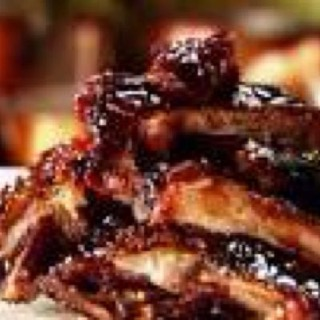
\includegraphics[width=0.9\linewidth]{/home/tim/Documents/projects/recipes/img/8046BA7D-6BD0-4D87-A0B7-3EC284E1A15A.jpg}\\
\end{minipage}\vspace{3mm}
\textbf{Directions}:
\vspace{-3mm}\begin{enumerate}\setlength\itemsep{-1mm}
\item Pour sauce on ribs or chicken. Cook at 325 for 2 hours. Turn off oven and let sit.
\end{enumerate}
\end{minipage}\vspace{8mm}
\noindent\begin{minipage}[t]{\linewidth}%
{\Large\textbf{Sausage Balls}} \label{sausage-balls}\hfill\textit{Sue Dunn}\\
\noindent\begin{minipage}[t]{0.78\linewidth}%
\textbf{Ingredients}:\vspace{-3mm}
\begin{multicols}{2}
\begin{itemize}\setlength\itemsep{-1mm}
\item 2 cups bisquick
\item 1 sausage
\item 12 oz sharp cheddar cheese
\end{itemize}
\end{multicols}
\end{minipage}
\noindent\begin{minipage}[t]{0.18\linewidth}
\centering \strut\vspace*{-\baselineskip}\newline
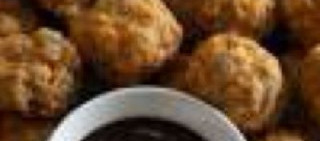
\includegraphics[width=0.9\linewidth]{/home/tim/Documents/projects/recipes/img/9A973527-B47D-4EBC-8158-F139E77AAE4E.jpg}\\
\end{minipage}\vspace{3mm}
\textbf{Directions}:
\vspace{-3mm}\begin{enumerate}\setlength\itemsep{-1mm}
\item Mix ingredients. Bake at 350 degrees for 10 minutes. Freeze. Reheat 10-15 minutes at 350 degrees.
\end{enumerate}
\end{minipage}\vspace{8mm}
\noindent\begin{minipage}[t]{\linewidth}%
{\Large\textbf{Southern Succor Rub}} \label{southern-succor-rub}\hfill\textit{Uncle Tim Dunn}\\
\textbf{Yield:} \textit{enough rub for one pork butt, with some left over}\\
\noindent\begin{minipage}[t]{0.78\linewidth}%
\textbf{Ingredients}:\vspace{-3mm}
\begin{multicols}{2}
\begin{itemize}\setlength\itemsep{-1mm}
\item 1/4 cup ground black pepper
\item 1/4 cup paprika
\item 1/4 cup Turbinado/'Sugar in the Raw'/Demerara Sugar
\item 2 Tbsp table salt
\item 2 tsp dry mustard
\item 1 tsp cayenne pepper
\end{itemize}
\end{multicols}
\end{minipage}
\noindent\begin{minipage}[t]{0.18\linewidth}
\centering \strut\vspace*{-\baselineskip}\newline
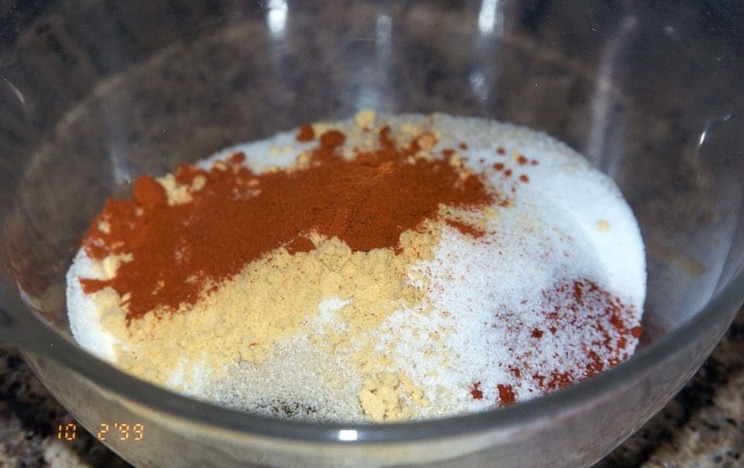
\includegraphics[width=0.9\linewidth]{/home/tim/Documents/projects/recipes/img/pork_rub.jpg}\\
\end{minipage}\vspace{3mm}
\textbf{Directions}:
\vspace{-3mm}\begin{enumerate}\setlength\itemsep{-1mm}
\item Mix ingredients thoroughly.
\end{enumerate}
\end{minipage}\vspace{8mm}

{\newpage \LARGE \textbf{Chicken}} \label{chicken}\\
\noindent\begin{minipage}[t]{\linewidth}%
{\Large\textbf{Broccoli Chicken Casserole}} \label{broccoli-chicken-casserole}\hfill\textit{Nancy Feth}\\
\noindent\begin{minipage}[t]{0.78\linewidth}%
\textbf{Ingredients}:\vspace{-3mm}
\begin{multicols}{2}
\begin{itemize}\setlength\itemsep{-1mm}
\item 2 (10 oz) packages proccoli cuts
\item 3 whole chicken breasts (cooked, boned and cut in pieces)
\item 2 cans condensed cream of chicken soup
\item 1 cup mayonnaise
\item 1 tsp lemon juice
\item 1/2 tsp curry powder
\item 1 cup shredded sharp cheddar cheese
\end{itemize}
\end{multicols}
\end{minipage}
\noindent\begin{minipage}[t]{0.18\linewidth}
\centering \strut\vspace*{-\baselineskip}\newline
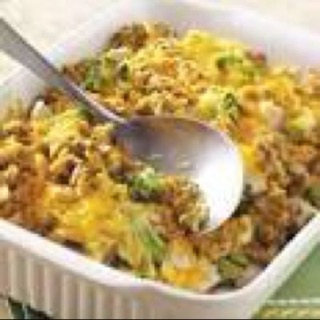
\includegraphics[width=0.9\linewidth]{/home/tim/Documents/projects/recipes/img/B22FE9D1-F626-4C5B-B0BD-B4F423DB41FA.jpg}\\
\end{minipage}\vspace{3mm}
\textbf{Directions}:
\vspace{-3mm}\begin{enumerate}\setlength\itemsep{-1mm}
\item Place uncooked broccoli in 9x13 baking dish. Season with salt and pepper.
\item Place cut-up chicken pieces on top. Make a sauce with soup, mayonnaise, lemon juice and curry powder. Pour over chicken. Sprinkle with cheese.
\item Bake for 30 minutes at 350F
\item If made 1 day in advance, refrigerate and bake slightly longer
\end{enumerate}
\end{minipage}\vspace{8mm}
\noindent\begin{minipage}[t]{\linewidth}%
{\Large\textbf{Chicken Cordon Bleu}} \label{chicken-cordon-bleu}\hfill\textit{Sue Dunn}\\
\noindent\begin{minipage}[t]{0.78\linewidth}%
\textbf{Ingredients}:\vspace{-3mm}
\begin{multicols}{2}
\begin{itemize}\setlength\itemsep{-1mm}
\item 6 boneless skinless chicken breast halves
\item 6 slices of swiss cheese
\item 6 slices of maple ham
\item 3 Tbsp all-purpose flour
\item 1 tsp paprika
\item 6 Tbsp butter
\item 1/2 cup dry white wine
\item 1 tsp chicken boullion (1 cube)
\item 1 Tbsp corn starch
\item 1 cup heavy whipping cream
\end{itemize}
\end{multicols}
\end{minipage}
\noindent\begin{minipage}[t]{0.18\linewidth}
\centering \strut\vspace*{-\baselineskip}\newline

\includegraphics[width=0.9\linewidth]{/home/tim/Documents/projects/recipes/img/none.jpg}\\
\end{minipage}\vspace{3mm}
\textbf{Directions}:
\vspace{-3mm}\begin{enumerate}\setlength\itemsep{-1mm}
\item Pound chicken breasts if too thick. Place cheese and ham on each breast. Fold chicken over filling and secure with toothpicks. Mix the flour and paprika in a small bowl and coat the chicken pieces.
\item Heat the butter in a large skillet over medium-high heat and cook the chicken until browned on all sides. Add the wine and bouillon. Reduce heat to low, cover and simmer for 30 minutes until chicken is no longer pink.
\item Remove the toothpicks and transfer the breasts to a warm platter. Blend cornstarch with cream in a small bowl and whisk slowly into skillet. Cook, stirring until thickened, and pour over chicken. Serve warm. 
\end{enumerate}
\end{minipage}\vspace{8mm}
\noindent\begin{minipage}[t]{\linewidth}%
{\Large\textbf{Chicken Devan}} \label{chicken-devan}\hfill\textit{Nancy Feth}\\
\noindent\begin{minipage}[t]{0.78\linewidth}%
\textbf{Ingredients}:\vspace{-3mm}
\begin{multicols}{2}
\begin{itemize}\setlength\itemsep{-1mm}
\item 2 pkg broccoli cuts
\item 3 whole chicken breasts (cooked, boned and cut in pieces)
\item 2 cans condensed cream of chicken soup
\item 1 cup mayonnaise
\item 1 tsp lemon juice
\item 1/2 tsp curry powder
\item 1 cup shredded cheddar cheese
\end{itemize}
\end{multicols}
\end{minipage}
\noindent\begin{minipage}[t]{0.18\linewidth}
\centering \strut\vspace*{-\baselineskip}\newline
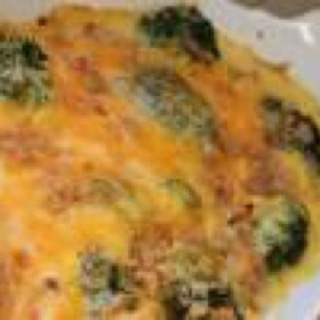
\includegraphics[width=0.9\linewidth]{/home/tim/Documents/projects/recipes/img/BEFEED18-A837-4235-853D-6933B6FB94FE.jpg}\\
\end{minipage}\vspace{3mm}
\textbf{Directions}:
\vspace{-3mm}\begin{enumerate}\setlength\itemsep{-1mm}
\item Place broccoli in 9x13 pan season with salt and pepper. Place chicken on top, make a sauce of soup, mayo, lemon juice and curry. Pour over above, sprinkle with cheese.
\item Bake 30 mins at 350
\end{enumerate}
\end{minipage}\vspace{8mm}
\noindent\begin{minipage}[t]{\linewidth}%
{\Large\textbf{Chicken Enchiladas}} \label{chicken-enchiladas}\hfill\textit{Sue Dunn}\\
\textbf{Yield:} \textit{4 servings}\\
\noindent\begin{minipage}[t]{0.78\linewidth}%
\textbf{Ingredients}:\vspace{-3mm}
\begin{multicols}{2}
\begin{itemize}\setlength\itemsep{-1mm}
\item 1 small onion, chopped
\item vegetable oil
\item 2 small cloves garlic, minced
\item 1 (15.5 oz) can roasted tomatoes
\item 2 Tbsp red chili powder
\item 1 tsp sugar
\item 1/2 to a cup of water
\item 12 corn tortillas
\item 2 cups of cooked chicken, shredded or chopped
\item salt
\item 2 cups grated cheese
\end{itemize}
\end{multicols}
\end{minipage}
\noindent\begin{minipage}[t]{0.18\linewidth}
\centering \strut\vspace*{-\baselineskip}\newline
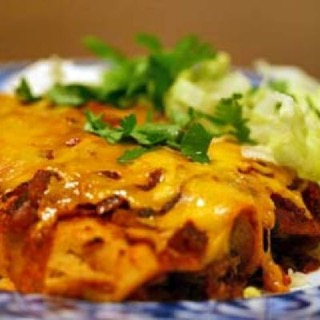
\includegraphics[width=0.9\linewidth]{/home/tim/Documents/projects/recipes/img/FF7A35FC-D2F8-4181-B882-42AA5ADC8179.jpg}\\
\end{minipage}\vspace{3mm}
\textbf{Directions}:
\vspace{-3mm}\begin{enumerate}\setlength\itemsep{-1mm}
\item Preheat the oven to 350F.
\item Prepare the sauce: Coat a large skillet with oil and saut the onions on medium heat until translucent, a few minutes. Add the garlic for a minute more. While the onions are cooking, puree the canned tomatoes in a blender. Add the tomatoes to the onions and garlic. Bring to a low simmer. Start adding the chili powder, one teaspoon at a time, tasting after each addition, until you get to the desired level of heat and chili flavor. For us that's around 2 Tablespoons. But it depends on your taste and how strong the chili powder is that you are using. Note that the tortillas and chicken will absorb some of the heat, so allow for that and let it be a little bit spicier than what you want in the finished dish. Add a teaspoon of sugar if necessary to cut down on the acid from the tomatoes. You want more of the taste of the chili and less of the tomatoes for this sauce. As the sauce simmers, dilute it with water to keep it from getting too thick as it simmers. Remove from heat.
\item Alternatively, use a prepared canned enchilada sauce, which can be perfectly fine.
\item Mix in 1/4 cup of the sauce with the cooked chicken, and a 1/4 cup of the cheese. Sprinkle with a little salt. Set aside.
\item Prepare the tortillas. There are 2 basic ways to prepare the tortillas - the traditional way of dipping them in the sauce and heating them individually, and my mom's way when she is trying to cut down on the fat.
\item First the traditional way. Heat a small light skillet on med-high heat. Add a teaspoon of oil (high smoke point oil as indicated above, we use grapeseed oil) to coat the pan. Dip a tortilla in the sauce to coat the tortilla with sauce on both sides. Place the tortilla in the skillet and heat for a few seconds, until the tortilla begin to show some air bubbles. Use a metal spatula to flip to the other side for a few more seconds. Set aside on a plate. Repeat with remaining tortillas. Proceed to the step 5.
\item For my mom's low-fat method of heating up the tortillas, she places a small amount of oil in the skillet to coat the pan. Add a tortilla, flip it to its other side. Then add another tortilla on top of the first to soak up some of the excess oil. Flip them both together and add yet another tortilla. Keep adding them wherever there seems to be some excess oil. The idea is to heat the tortillas and soften them with the minimum amount of oil. As the tortillas become soft and heated, remove them to a paper towel to soak up even more excess oil. If you find you need more oil in the pan, add it. With this method, you do NOT get the chili flavor infused in the tortillas. It is a matter of preference. I prefer the first method, excess oil or not, because it has a much richer and spicier flavor. But as my mom says, "Anything goes. This is just a guideline; do what you want." 
\item Note that because we made this batch the low-fat way, the following photos show tortillas not coated in chili sauce, but the method is the same for if you did.
\item  
\item 5 Assemble the enchiladas. Use an 8x12 inch pyrex baking dish. Place a couple spoonfuls of the chicken mixture in the center of a tortilla and roll it up. Place in the baking dish and repeat until all dozen of your tortillas are neatly placed in rows in the casserole dish. Cover the tortillas rolls with the remaining sauce. Sprinkle with the remaining grated cheese. Note that I recall often eating these chicken enchiladas with very little cheese on them. Instead we had probably 2/3 cup of chopped fresh onion that had been soaked in vinegar sprinkled over the top. (My mom, bless her soul, has no recollection of the chicken enchiladas without the sprinkled cheese. But she's in her 70s and sometimes doesn't remember these things. Or she remembers later and doesn't remember that she ever forgot them in the first place. But heck, I'm in my 40s and my memory isn't what it used to be either.)
\item Place in the oven and cook for 10 minutes, or until cheese is bubbly.
\item Use a metal spatula to serve.
\item Serve with thinly sliced iceberg lettuce that has been seasoned with vinegar and salt (no oil), guacamole or avocado slices, and sour cream. Garnish with cilantro.
\end{enumerate}
\end{minipage}\vspace{8mm}
\noindent\begin{minipage}[t]{\linewidth}%
{\Large\textbf{Chicken and Artichoke Bake}} \label{chicken-and-artichoke-bake}\hfill\textit{Sue Dunn}\\
\noindent\begin{minipage}[t]{0.78\linewidth}%
\textbf{Ingredients}:\vspace{-3mm}
\begin{multicols}{2}
\begin{itemize}\setlength\itemsep{-1mm}
\item 1 (14 oz) can water-packed artichokes
\item 3/4 cup grated parmesan cheese
\item 3/4 cup light mayonnaise
\item garlic powder
\item 6 skinless boneless chicken breasts, cut lengthwise in half
\end{itemize}
\end{multicols}
\end{minipage}
\noindent\begin{minipage}[t]{0.18\linewidth}
\centering \strut\vspace*{-\baselineskip}\newline

\includegraphics[width=0.9\linewidth]{/home/tim/Documents/projects/recipes/img/none.jpg}\\
\end{minipage}\vspace{3mm}
\textbf{Directions}:
\vspace{-3mm}\begin{enumerate}\setlength\itemsep{-1mm}
\item Drain artichokes. Squeeze all water out of each artichoke. Chop.
\item Combine artichokes, cheese, mayo, and garlic in a bowl. Mix thoroughly.
\item Place chicken in a greased 11 x 7 inch baking dish. Spread artichoke mixture over chicken. Bake uncovered at 375F for 30-35 minutes.
\end{enumerate}
\end{minipage}\vspace{8mm}
\noindent\begin{minipage}[t]{\linewidth}%
{\Large\textbf{Chile, Chicken, and Cheese Casserole}} \label{chile,-chicken,-and-cheese-casserole}\hfill\textit{Andrew Kulawiec}\\
\noindent\begin{minipage}[t]{0.78\linewidth}%
\textbf{Ingredients}:\vspace{-3mm}
\begin{multicols}{2}
\begin{itemize}\setlength\itemsep{-1mm}
\item 12-16 small flour tortillas
\item 16 oz sour cream
\item 2 cans condensed cream of chicken soup
\item 1 lb Cooked chicken
\item 2 small cans of chopped green chilies
\item 1 block extra sharp cheddar cheese
\item Monterey jack cheese (optional)
\end{itemize}
\end{multicols}
\end{minipage}
\noindent\begin{minipage}[t]{0.18\linewidth}
\centering \strut\vspace*{-\baselineskip}\newline
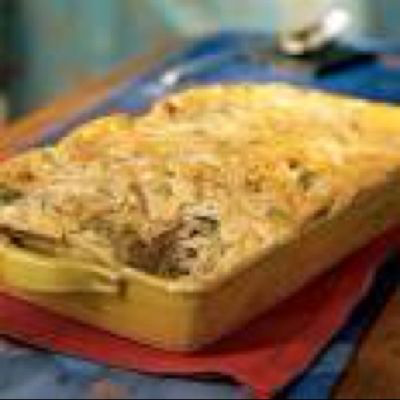
\includegraphics[width=0.9\linewidth]{/home/tim/Documents/projects/recipes/img/F6769DDE-B871-4966-97FC-4D0ABF315688.jpg}\\
\end{minipage}\vspace{3mm}
\textbf{Directions}:
\vspace{-3mm}\begin{enumerate}\setlength\itemsep{-1mm}
\item Layer Twice: tortillas to cover the bottom of a 9x13 pan, cream of chicken soup, chicken, sour cream, chiles, cheese.
\item Bake at 325F for 25 minutes. Then turn to 350F until golden brown.
\end{enumerate}
\end{minipage}\vspace{8mm}
\noindent\begin{minipage}[t]{\linewidth}%
{\Large\textbf{Cream Cheese Spinach Stuffed Chicken}} \label{cream-cheese-spinach-stuffed-chicken}\hfill\textit{Sue Dunn}\\
\textit{``Chicken breasts stuffed with a creamy spinach, parmesan, mozerella, and cream cheese filling and pan seared to perfection.''}\\
\textbf{Yield:} \textit{8 servings}\\
\noindent\begin{minipage}[t]{0.78\linewidth}%
\textbf{Ingredients}:\vspace{-3mm}
\begin{multicols}{2}
\begin{itemize}\setlength\itemsep{-1mm}
\item 8 (4 oz) chicken breasts
\item 2 tsp chili powder
\item 2 tsp Italian seasoning
\item 1 tsp black pepper
\item 1 tsp salt
\item 1 Tbsp olive oil
\item 4 cups spinach (or one 10 oz package, thawed and drained)
\item 8 oz cream cheese (room temp)
\item 0.5 cup Parmesan cheese
\item 0.5 cup mozarella cheese
\item 2 Tbsp minced garlic
\item 0.5 tsp pepper
\item salt to taste
\end{itemize}
\end{multicols}
\end{minipage}
\noindent\begin{minipage}[t]{0.18\linewidth}
\centering \strut\vspace*{-\baselineskip}\newline

\includegraphics[width=0.9\linewidth]{/home/tim/Documents/projects/recipes/img/none.jpg}\\
\end{minipage}\vspace{3mm}
\textbf{Directions}:
\vspace{-3mm}\begin{enumerate}\setlength\itemsep{-1mm}
\item To make the filling: in a medium bowl, combine the spinach, cream cheese, parmesan cheese, mozzarella cheese, garlic, salt, and pepper.
\item To butterfly the chicken breasts: lay them flat on a sturdy surface. Place one hand on top to hold it in place and slice 3/4 of the way through the chicken breast.
\item To stuff the chicken: season the outside of the chicken with chili powder, Italian seasoning, salt, and pepper. Spoon 1/4 of the cheese mixture into the middle of the cut chicken breasts and fold the chicken so the cream cheese is sealed inside. Use toothpicks if necessary.
\item To cook: Heat a non-stick skillet on medium-high and add olive oil. Cook the chicken, covering the pan with a lid, for about 9-10 minutes per side or until the chicken is cooked through.
\end{enumerate}
\end{minipage}\vspace{8mm}
\noindent\begin{minipage}[t]{\linewidth}%
{\Large\textbf{Oriental Chicken Salad}} \label{oriental-chicken-salad}\hfill\textit{Lynn Neff}\\
\noindent\begin{minipage}[t]{0.78\linewidth}%
\textbf{Ingredients}:\vspace{-3mm}
\begin{multicols}{2}
\begin{itemize}\setlength\itemsep{-1mm}
\item 1 cooked chicken, shredded
\item 1/2 package wonton shells, cut in 1/4 inch strips and fried in peanut oil
\item 2 heads lettuce, shredded
\item 8 green onions, sliced
\item 4 tsp sliced almonds, toasted
\item 4 Tbsp sesame seeds
\item 1/2 cup white vinegar
\item 1/2 cup ketchup
\item 1/2 cup water
\item 12 Tbsp sugar
\item 2 tsp soy
\end{itemize}
\end{multicols}
\end{minipage}
\noindent\begin{minipage}[t]{0.18\linewidth}
\centering \strut\vspace*{-\baselineskip}\newline
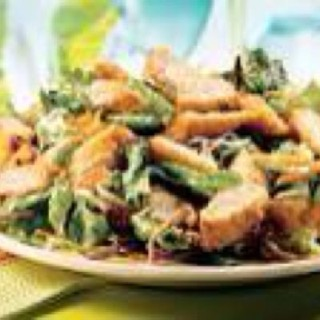
\includegraphics[width=0.9\linewidth]{/home/tim/Documents/projects/recipes/img/208306E3-ECAD-4693-8AA9-7461D5210B63.jpg}\\
\end{minipage}\vspace{3mm}
\textbf{Directions}:
\vspace{-3mm}\begin{enumerate}\setlength\itemsep{-1mm}
\item Tap and Hold image
\item Touch 'Save Image' to save the image to your iPad
\item Tap here to open app importer.
\item Once the app opens and imports the recipe, upload the picture you saved from the email (iPad app only)
\end{enumerate}
\end{minipage}\vspace{8mm}
\noindent\begin{minipage}[t]{\linewidth}%
{\Large\textbf{Seared Chicken With Avocado}} \label{seared-chicken-with-avocado}\hfill\textit{allrecipes.com}\\
\noindent\begin{minipage}[t]{0.78\linewidth}%
\textbf{Ingredients}:\vspace{-3mm}
\begin{multicols}{2}
\begin{itemize}\setlength\itemsep{-1mm}
\item 1 1/2 tsp blackened seasoning
\item 4 (4 oz) skinless, boneless chicken breast halves
\item 1 tsp olive oil
\item 1 diced, peeled avocado
\item 2 Tbsp chopped fresh cilantro
\item 1 jalapeno pepper, seeded and finely chopped
\item 2 Tbsp freh lime juice (anout 1 lime)
\item 1/4 tsp salt
\item 1 lime, cut into quarters
\end{itemize}
\end{multicols}
\end{minipage}
\noindent\begin{minipage}[t]{0.18\linewidth}
\centering \strut\vspace*{-\baselineskip}\newline
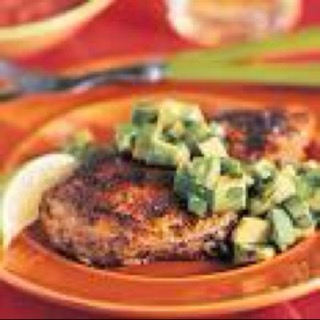
\includegraphics[width=0.9\linewidth]{/home/tim/Documents/projects/recipes/img/F487A08A-06D4-4929-8018-9121063658C4.jpg}\\
\end{minipage}\vspace{3mm}
\textbf{Directions}:
\vspace{-3mm}\begin{enumerate}\setlength\itemsep{-1mm}
\item Sprinkle seasoning on both sides of chicken
\item Heat oil in a large nonstick skillet over high heat. Add chicken, smooth side down, to pan; cook 1 minute or until seared.
\item Reduce hate to medium; cook 3 minutes on each side or until lightly browned.
\item Combine avocado, cilantro, pepper, lime juice and salt.
\item Squeeze one-quarter lime over each piece of chicken before serving. Serve with avocado mixture.
\end{enumerate}
\end{minipage}\vspace{8mm}
\noindent\begin{minipage}[t]{\linewidth}%
{\Large\textbf{Sour Cream Salsa Chicken}} \label{sour-cream-salsa-chicken}\hfill\textit{Sue Dunn}\\
\noindent\begin{minipage}[t]{0.78\linewidth}%
\textbf{Ingredients}:\vspace{-3mm}
\begin{multicols}{2}
\begin{itemize}\setlength\itemsep{-1mm}
\item 5 boneless chicken breasts
\item 1 package taco seasoning mix
\item 1 cup salsa
\item 2 Tbsp corn starch
\item 1/4 cup sour cream
\end{itemize}
\end{multicols}
\end{minipage}
\noindent\begin{minipage}[t]{0.18\linewidth}
\centering \strut\vspace*{-\baselineskip}\newline

\includegraphics[width=0.9\linewidth]{/home/tim/Documents/projects/recipes/img/none.jpg}\\
\end{minipage}\vspace{3mm}
\textbf{Directions}:
\vspace{-3mm}\begin{enumerate}\setlength\itemsep{-1mm}
\item Spray crockpot with cooking spray and line with chicken. Sprinkle taco mix on top and top with salsa, then cook on low for 6-8 hours.
\item Remove chicken from pot. Mix corn starch with a little water and add to salsa. Stir in sour cream.
\item Return chicken to pot for 30-45 more minutes or until hot again.
\end{enumerate}
\end{minipage}\vspace{8mm}

{\newpage \LARGE \textbf{Pastas}} \label{pastas}\\
\noindent\begin{minipage}[t]{\linewidth}%
{\Large\textbf{Cauliflower Casserole}} \label{cauliflower-casserole}\hfill\textit{Sue Dunn}\\
\textbf{Yield:} \textit{8 servings, 1/2 cup each}\\
\noindent\begin{minipage}[t]{0.78\linewidth}%
\textbf{Ingredients}:\vspace{-3mm}
\begin{multicols}{2}
\begin{itemize}\setlength\itemsep{-1mm}
\item 1 large head cauliflower, cut into small florets
\item 2 Tbsp butter, melted
\item sea salt
\item black pepper
\item 2/3 cup sour cream
\item 1/4 cup heavy cream
\item 2 cloves garlic, minced
\item 1 1/2 cup cheddar cheese (shredded)
\item 6 Tbsp bacon bits
\item 1/4 cup green onions
\end{itemize}
\end{multicols}
\end{minipage}
\noindent\begin{minipage}[t]{0.18\linewidth}
\centering \strut\vspace*{-\baselineskip}\newline
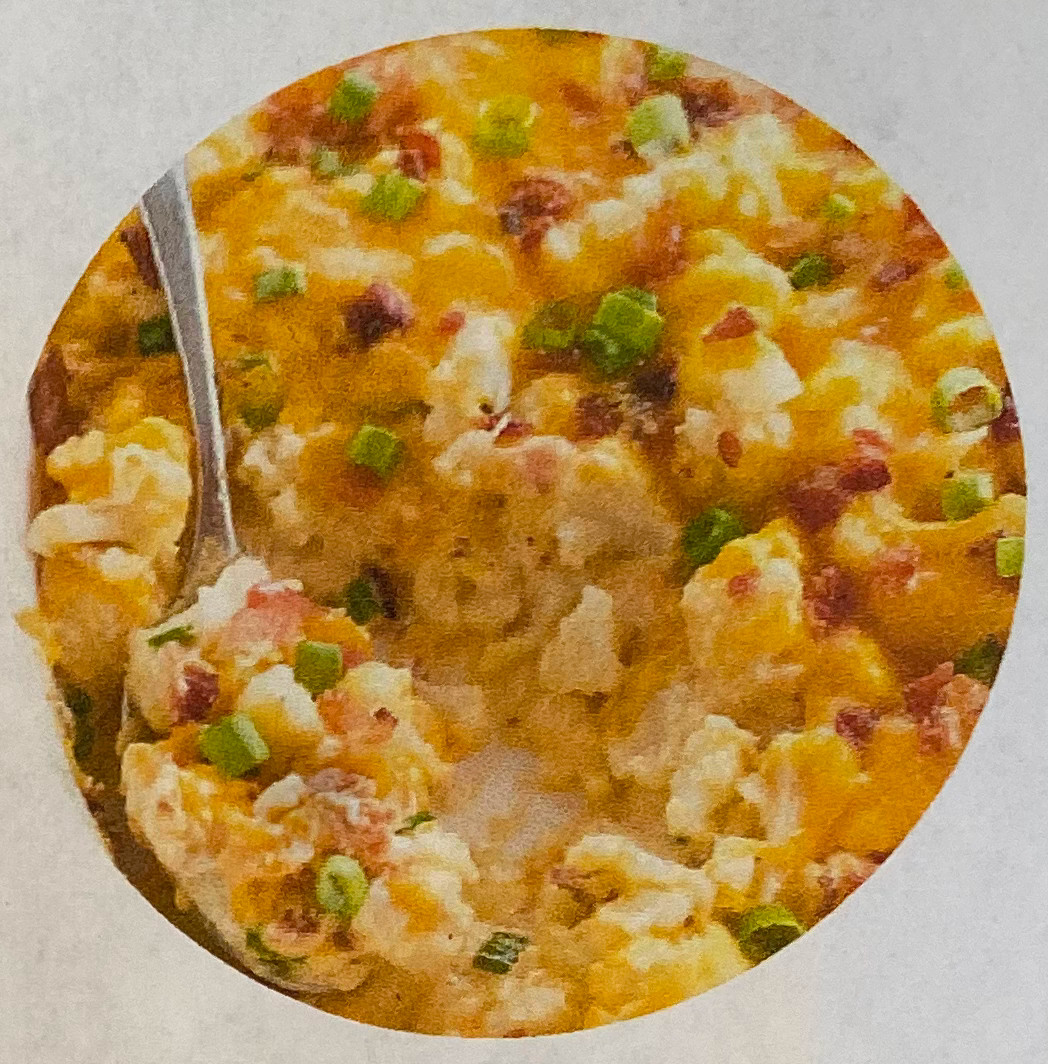
\includegraphics[width=0.9\linewidth]{/home/tim/Documents/projects/recipes/img/cauliflower.jpg}\\
\end{minipage}\vspace{3mm}
\textbf{Directions}:
\vspace{-3mm}\begin{enumerate}\setlength\itemsep{-1mm}
\item Preheat the oven to 450F.
\item In a large bowl, toss the cauliflower florets with butter. Season with salt and black pepper.
\item Roast on a baking sheet for 15-20 minutes, until crisp and tender.
\item Meanwhile, in the same bowl, whisk together the sour and heavy creams, until smooth. Stir in the minced garlic, half of the cheddar cheese, half of the bacon bits, and half of the green onions. If desired, season sauce with sea salt and black pepper (keep in mind, the cheese will make it saltier as it melts).
\item When the cauliflower is done roasting, take it out and leave the oven on. Add the cauliflower to the bowl and mix with the sauce. Transfer to the casserole dish, and top with the remaining cheese and bacon bits.
\item Bake for 5-10 minutes, until the cheese melts. Top with remaining green onions.
\end{enumerate}
\end{minipage}\vspace{8mm}
\noindent\begin{minipage}[t]{\linewidth}%
{\Large\textbf{Mac and Cheese}} \label{mac-and-cheese}\hfill\textit{Tim Dunn}\\
\noindent\begin{minipage}[t]{0.78\linewidth}%
\textbf{Ingredients}:\vspace{-3mm}
\begin{multicols}{2}
\begin{itemize}\setlength\itemsep{-1mm}
\item 8 oz uncooked elbow macaroni
\item 2 cups shredded sharp cheddar cheese
\item 1/2 cup grated parmesan cheese
\item 3 cups milk
\item 1/4 cup butter
\item 2 1/2 Tbsp all-purpose flour
\item 2 Tbsp butter
\item 1/2 cup bread crumbs
\item 1 pinch paprika
\end{itemize}
\end{multicols}
\end{minipage}
\noindent\begin{minipage}[t]{0.18\linewidth}
\centering \strut\vspace*{-\baselineskip}\newline
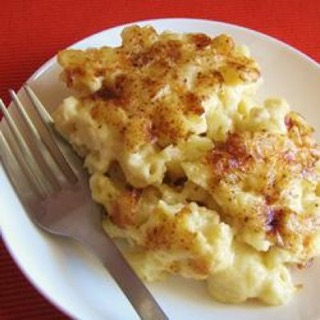
\includegraphics[width=0.9\linewidth]{/home/tim/Documents/projects/recipes/img/5912D818-08DA-4FC5-9BD6-33E9D7C12A43.jpg}\\
\end{minipage}\vspace{3mm}
\textbf{Directions}:
\vspace{-3mm}\begin{enumerate}\setlength\itemsep{-1mm}
\item Cook macaroni; drain.
\item In a saucepan, melt butter or margarine over medium heat. Stir in enough flour to make a roux. Add milk to roux slowly, stirring constantly. Stir in cheeses, and cook over low heat until cheese is melted and the sauce is a little thick. Put macaroni in large casserole dish, and pour sauce over macaroni. Stir well.
\item Melt butter or margarine in a skillet over medium heat. Add breadcrumbs and brown. Spread over the macaroni and cheese to cover. Sprinkle with a little paprika.
\item Bake at 350F for 30 minutes.
\end{enumerate}
\end{minipage}\vspace{8mm}
\noindent\begin{minipage}[t]{\linewidth}%
{\Large\textbf{Spaghetti Squash Gratin}} \label{spaghetti-squash-gratin}\hfill\textit{Sue Dunn}\\
\textbf{Yield:} \textit{5 cups}\\
\noindent\begin{minipage}[t]{0.78\linewidth}%
\textbf{Ingredients}:\vspace{-3mm}
\begin{multicols}{2}
\begin{itemize}\setlength\itemsep{-1mm}
\item 1 (2-3 lb) spaghetti squash, halved and seeded
\item 1 clove garlic, chopped
\item 1 Tbsp fresh thyme
\item 2 Tbsp fresh parsley
\item 1/2 tsp salt
\item 1/4 tsp fresh cracked pepper
\item 1 (8 oz) pkg creme fraiche
\item 1 cup shredded asiago cheese
\end{itemize}
\end{multicols}
\end{minipage}
\noindent\begin{minipage}[t]{0.18\linewidth}
\centering \strut\vspace*{-\baselineskip}\newline
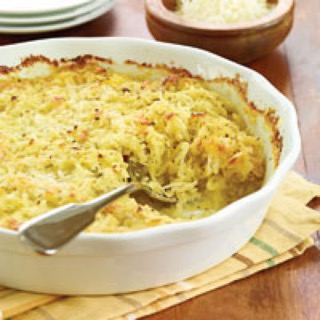
\includegraphics[width=0.9\linewidth]{/home/tim/Documents/projects/recipes/img/D7FA3935-A406-4952-9C6A-CFFC0F7BC23F.jpg}\\
\end{minipage}\vspace{3mm}
\textbf{Directions}:
\vspace{-3mm}\begin{enumerate}\setlength\itemsep{-1mm}
\item Preheat oven to 450 degrees. 
\item Microwave squash (one half at a time, skin side up) on high until tender (10-12 minutes). Set aside, covered, until cool enough to handle (10-15 minutes).
\item Run tines of fork lengthwise over cut surface of squash to loosen spaghetti-like strands; scoop out strands. If necessary, drain excess liquid. Set aside. 
\item Combine garlic, thyme, parsley, salt, pepper, creme fraiche, and 2/3 cup cheese in small bowl. Fold into squash; place in casserole dish. Top with remaining cheese.
\item Bake 20 minutes or until lightly browned.
\end{enumerate}
\end{minipage}\vspace{8mm}

{\newpage \LARGE \textbf{Breads}} \label{breads}\\
\noindent\begin{minipage}[t]{\linewidth}%
{\Large\textbf{Amish Cinnamon Bread}} \label{amish-cinnamon-bread}\hfill\textit{}\\
\textit{``also known as 'friendship bread'''}\\
\noindent\begin{minipage}[t]{0.78\linewidth}%
\textbf{Ingredients}:\vspace{-3mm}
\begin{multicols}{2}
\begin{itemize}\setlength\itemsep{-1mm}
\item 2 1/2 Cups milk
\item 3 Cups sugar
\item 4 Cups flour
\item 1 Cup vegetable oil
\item 1/2 Cup milk
\item 3 eggs
\item 1 tsp vanilla
\item 2 tsp cinnamon
\item 1 box vanilla instant pudding mix (6 ounce)
\item 1/2 Cup nuts (optional)
\item 1/2 Cup raisins (optional)
\end{itemize}
\end{multicols}
\end{minipage}
\noindent\begin{minipage}[t]{0.18\linewidth}
\centering \strut\vspace*{-\baselineskip}\newline

\includegraphics[width=0.9\linewidth]{/home/tim/Documents/projects/recipes/img/none.jpg}\\
\end{minipage}\vspace{3mm}
\textbf{Directions}:
\vspace{-3mm}\begin{enumerate}\setlength\itemsep{-1mm}
\item Day One: For those making the starter from scratch: combine 1 cup milk, 1 cup sugar, and 1 cup flour in a large zip lock bag and mush to mix ingredients. For those receiving the fermented batter in a gallon zip lock bag: Do nothing. Leave it to sit on the counter.
\item On days 2-4: Squeeze the bag several times during the day. (If air builds up in the bag, open the zip lock slightly and remove the air). I took mine to work, laid it on my desk, and to relieve stress squeezed the bag several times during the day. Ha ha ha!
\item On day 5: add 1 cup milk, 1 cup sugar, and 1 cup self-rising flour to the bag. Squeeze the bag several times during the day.
\item On days 6-8: Squeeze the bag several times during the day.(remove air).
\item On day 9: Add 1 cup milk, 1 cup sugar, and 1 cup self-rising flour into the bag. Close zip lock. Squeeze the bag several times during the day.
\item Day 10: Pour 1/2 cup "starter" in four (4) separate gallon zip lock bags. These starters replace the milk, flour, and sugar used to start the very first batch from scratch. Give the four bags to friends along with the steps on how to finish making their own starters and bread, or freeze the starters for future use if desired, just be sure that once you take a starter out of the freezer, you let it sit out one day before starting your steps.
\item In a large glass bowl add 2 cups self-rising flour, 1 cup of sugar, 3 eggs, 1 cup oil, 2 tsp cinnamon, 1/2 cup milk, 1 tsp vanilla, 1 large box (or 2 small boxes) of instant vanilla pudding, 1/2 cup of either raisins, nuts, chocolate chips or fruit (optional) or 1/4 cup of any two of these ingredients; mix well.
\item Spray well 2 large loaf pans with cooking spray.
\item In a small bowl or cup, mix 1 tsp cinnamon and 2 tbsp sugar. Sprinkle about 1/2 to 2/3 in loaf pans, reserving about 1/3 to 1/2 of the mix.
\item Pour batter into pans.
\item Sprinkle remaining cinnamon and sugar mix across the tops of the batter.(You may choose to sprinkle the remaining mix after baking the bread).
\item Bake at 325 degrees for 1 hour.
\item IMPORTANT NOTES:
\item You may also make small loaves. If you do, bake at the same temperature, but for 25-30 minutes.
\item Do not use metal spoon or metal bowl for mixing.
\item Do not refrigerate at any time during the process. Keep on the counter.
\item If air builds up in the zip lock. Open the zipper slightly and squeeze the air out, being careful not to let any of the batter out. Quickly reseal.
\item It is normal for the batter to thicken and bubble during the time it sits on the counter. This is called the fermentation process.
\item You may replace the nuts or the raisins with chocolate chips or dried fruit (or fresh, not canned or frozen). Or you can eliminate them and just leave it plain. It's great any way you slice it. ;0).
\item Also, the bread will yield more than four serving. If you do the two large loafs, it will yield how ever large a slice you want it to be. So if sliced about the size of a normal slice of bread, one loaf could yield about 16-18 slices. The serving size listed came off the paper I got with the recipe. I'm not sure why they say four servings. Each of four servings would be 1/2 a loaf.
\end{enumerate}
\end{minipage}\vspace{8mm}
\noindent\begin{minipage}[t]{\linewidth}%
{\Large\textbf{Apple Wheat Bread}} \label{apple-wheat-bread}\hfill\textit{Sue Dunn}\\
\textit{``Shredded apple in this mild, wheaty bread adds an elusive flavor and keeps it moist.''}\\
\textbf{Yield:} \textit{2 loaves}\\
\noindent\begin{minipage}[t]{0.78\linewidth}%
\textbf{Ingredients}:\vspace{-3mm}
\begin{multicols}{2}
\begin{itemize}\setlength\itemsep{-1mm}
\item 1 package active dry yeast
\item 1 1/4 cups warm (105-115F) water
\item 1/4 cup firmly packed brown sugar
\item 1 cup warm (105-115F) milk
\item 1 1/2 tsp salt
\item 2 Tbsp salad oil
\item 5 cups unbleached all-purpose flour
\item 1 1/2 cups whole wheat flour
\item 1 large apple, peeled, cored, and shredded
\end{itemize}
\end{multicols}
\end{minipage}
\noindent\begin{minipage}[t]{0.18\linewidth}
\centering \strut\vspace*{-\baselineskip}\newline

\includegraphics[width=0.9\linewidth]{/home/tim/Documents/projects/recipes/img/none.jpg}\\
\end{minipage}\vspace{3mm}
\textbf{Directions}:
\vspace{-3mm}\begin{enumerate}\setlength\itemsep{-1mm}
\item Sprinkle yeast over 1/4 cup of the water in a large bowl or electric mixer. Add 1 tsp of the brown sugar. Let stand until soft (5 minutes).
\item Stir in remaining water, milk, remaining brown sugar, salt, and oil.
\item Add 3 1/2 cups of the unbleached flour. Mix to blend, then beat at medium speed until smooth and elastic (5 minutes). Stir in whole wheat flour and apple. Then stir in about 3/4 cup more unbleached flour to make a soft dough.
\item Turn dough out onto a board or pastry cloth coated with some of the remaining 3/4 cup unbleached flour. Knead until dough is smooth and springy and small bubbles form just under surface (12-15 minutes), adding just enough flour to prevent dough from being sticky.
\item Turn dough in a greased bowl. Cover with plastic wrap and a towel; let rise in a warm place until doubled in bulk (1 1/4 - 1 1/2 hours).
\item Punch dough down and divide into two equal portions. Shape each into a loaf. Place loaves in greased 4 1/2 x 8 1/2 inch loaf pans. Let rise until almost doubled in bulk (40-45 minutes).
\item Preheat oven to 350F. Bake until loaves are well browned and sound hollow when tapped (40-45 minutes). Remove loaves from pans and let cool on wire racks.
\end{enumerate}
\end{minipage}\vspace{8mm}
\noindent\begin{minipage}[t]{\linewidth}%
{\Large\textbf{Banana Bread}} \label{banana-bread}\hfill\textit{Alpha Bakery Children's Book}\\
\noindent\begin{minipage}[t]{0.78\linewidth}%
\textbf{Ingredients}:\vspace{-3mm}
\begin{multicols}{2}
\begin{itemize}\setlength\itemsep{-1mm}
\item 3/4 cup sugar
\item 1 1/2 cups mashed bananas (3 large)
\item 3/4 cup vegetable oil
\item 2 eggs
\item 2 cups all-purpose flour
\item 1/2 cup chocolate chips
\item 1 tsp baking soda
\item 2 tsp vanilla
\item 1/2 tsp baking powder
\item 1/2 tsp salt
\end{itemize}
\end{multicols}
\end{minipage}
\noindent\begin{minipage}[t]{0.18\linewidth}
\centering \strut\vspace*{-\baselineskip}\newline
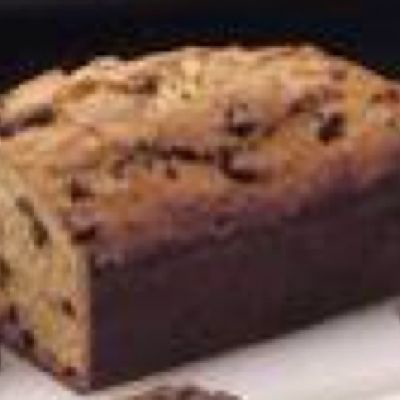
\includegraphics[width=0.9\linewidth]{/home/tim/Documents/projects/recipes/img/A1DC5656-FAA8-460B-9E34-05D4EEAB7F19.jpg}\\
\end{minipage}\vspace{3mm}
\textbf{Directions}:
\vspace{-3mm}\begin{enumerate}\setlength\itemsep{-1mm}
\item Heat the oven to 350F.
\item Grease a loaf pan, either 9x5x3 or 8 1/2 x4 1/2 x2 1/2 inches, with shortening, using a pastry brush.
\item Mix sugar, bananas, oil and eggs in a large bowl with a wooden spoon. Stir in remaining ingredients. Pour into pan.
\item Bake until a wooden pick inserted in the center of the bread comes out clean (60-70 minutes). Let cool 10 minutes, then loosen sides of loaf from pan and remove from pan. Let cool completely before slicing. 
\end{enumerate}
\end{minipage}\vspace{8mm}
\noindent\begin{minipage}[t]{\linewidth}%
{\Large\textbf{Zucchini Bread}} \label{zucchini-bread}\hfill\textit{allrecipes.com}\\
\noindent\begin{minipage}[t]{0.78\linewidth}%
\textbf{Ingredients}:\vspace{-3mm}
\begin{multicols}{2}
\begin{itemize}\setlength\itemsep{-1mm}
\item 3 cups all-purpose flour
\item 1 tsp salt
\item 1 tsp baking soda
\item 1 tsp baking powder
\item 3 tsp ground cinnamon
\item 3 eggs
\item 1 cup vegetable oil
\item 2 1/4 cups white sugar
\item 3 tsp vanilla extract
\item 2 cups grated zucchini
\item 1 cup chopped walnuts
\end{itemize}
\end{multicols}
\end{minipage}
\noindent\begin{minipage}[t]{0.18\linewidth}
\centering \strut\vspace*{-\baselineskip}\newline
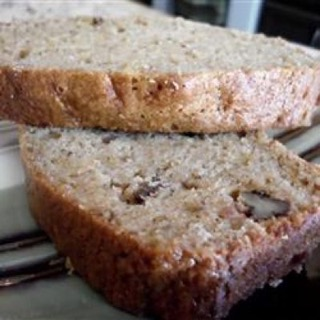
\includegraphics[width=0.9\linewidth]{/home/tim/Documents/projects/recipes/img/3671A514-1C82-49BB-B842-F8A855CF46B6.jpg}\\
\end{minipage}\vspace{3mm}
\textbf{Directions}:
\vspace{-3mm}\begin{enumerate}\setlength\itemsep{-1mm}
\item Grease and flour two 8 x 4 inch pans. Preheat oven to 325 degrees F (165 degrees C).
\item Sift flour, salt, baking powder, soda, and cinnamon together in a bowl.
\item Beat eggs, oil, vanilla, and sugar together in a large bowl. Add sifted ingredients to the creamed mixture, and beat well. Stir in zucchini and nuts until well combined. Pour batter into prepared pans.
\item Bake for 40 to 60 minutes, or until tester inserted in the center comes out clean. Cool in pan on rack for 20 minutes. Remove bread from pan, and completely cool.
\end{enumerate}
\end{minipage}\vspace{8mm}

{\newpage \LARGE \textbf{Pies}} \label{pies}\\
\noindent\begin{minipage}[t]{\linewidth}%
{\Large\textbf{Grasshopper Pie}} \label{grasshopper-pie}\hfill\textit{Sue Dunn}\\
\noindent\begin{minipage}[t]{0.78\linewidth}%
\textbf{Ingredients}:\vspace{-3mm}
\begin{multicols}{2}
\begin{itemize}\setlength\itemsep{-1mm}
\item 25 oreos
\item 1/2 cup butter, melted
\item 2 cups marshmallow creme (Fluff)
\item 1/4 cup Creme de Menthe liqueur
\item 2 cups whipping cream
\end{itemize}
\end{multicols}
\end{minipage}
\noindent\begin{minipage}[t]{0.18\linewidth}
\centering \strut\vspace*{-\baselineskip}\newline
\includegraphics[width=0.9\linewidth]{/home/tim/Documents/projects/recipes/img/CCDB5AC6-979A-4C68-8593-34CD428F0CBD.jpg}\\
\end{minipage}\vspace{3mm}
\textbf{Directions}:
\vspace{-3mm}\begin{enumerate}\setlength\itemsep{-1mm}
\item Crush cookies and set aside 1/4 cup of crumbs. Place remaining crumbs in a medium bowl and mix in melted butter. Press mixture firmly into bottom and sides of a 9 inch springform pan.
\item In a large mixing bowl, whip together marshmallow creme and creme de menthe until smooth. In a separate bowl, whip cream until soft peaks form, then fold into marshmallow mixture. Pour mixture into pan and sprinkle reserved cookie crumbs on top. Freeze at least 2 hours, until firm. Remove from freezer 20 minutes before serving to soften slightly.
\end{enumerate}
\end{minipage}\vspace{8mm}
\noindent\begin{minipage}[t]{\linewidth}%
{\Large\textbf{Pizza Bites}} \label{pizza-bites}\hfill\textit{Sue Dunn}\\
\noindent\begin{minipage}[t]{0.78\linewidth}%
\textbf{Ingredients}:\vspace{-3mm}
\begin{multicols}{2}
\begin{itemize}\setlength\itemsep{-1mm}
\item unknown
\end{itemize}
\end{multicols}
\end{minipage}
\noindent\begin{minipage}[t]{0.18\linewidth}
\centering \strut\vspace*{-\baselineskip}\newline
\includegraphics[width=0.9\linewidth]{/home/tim/Documents/projects/recipes/img/A8B5D904-A163-40ED-A6AF-9CA1CFB88DE0.jpg}\\
\end{minipage}\vspace{3mm}
\textbf{Directions}:
\vspace{-3mm}\begin{enumerate}\setlength\itemsep{-1mm}
\item unknown
\end{enumerate}
\end{minipage}\vspace{8mm}

{\newpage \LARGE \textbf{Cookies}} \label{cookies}\\
\noindent\begin{minipage}[t]{\linewidth}%
{\Large\textbf{Almond Macaroons}} \label{almond-macaroons}\hfill\textit{}\\
\noindent\begin{minipage}[t]{0.78\linewidth}%
\textbf{Ingredients}:\vspace{-3mm}
\begin{multicols}{2}
\begin{itemize}\setlength\itemsep{-1mm}
\item 10 oz blanched whole almonds (about 2 full cups)
\item 2 3/4 Cups granulated sugar
\item 3 Large egg whites
\item 1/2 tsp pure almond extract
\item 6 oz good quality bittersweet chocolate, chopped (optional)
\end{itemize}
\end{multicols}
\end{minipage}
\noindent\begin{minipage}[t]{0.18\linewidth}
\centering \strut\vspace*{-\baselineskip}\newline
\includegraphics[width=0.9\linewidth]{/home/tim/Documents/projects/recipes/img/DD993399-6C6B-4C84-ADE9-9D35E6F5E3F3.jpg}\\
\end{minipage}\vspace{3mm}
\textbf{Directions}:
\vspace{-3mm}\begin{enumerate}\setlength\itemsep{-1mm}
\item Preheat oven to 350 degrees. Line one or two cookie sheets with parchment paper.
\item Combine the almonds and 1/4 cup of the sugar in a food processor and process until the almonds are finely ground. Add the egg whites and almond extract and process until blended.
\item Add the remaining 1 cup of sugar and process until thoroughly combined, about 15 seconds, or until the dough is a thick, sticky paste.
\item Drop the dough by level tablespoonfuls, arranging about 2 inches apart on the prepared sheet(s). Using a pastry brush lightly moistened with water, brush the tops and sides of the macaroons, gently pressing down on them to form smooth rounds about 1/2 inch thick and 1 3/4 inches in diameter.
\item Bake for about 15 minutes or until the macaroons are pale golden. They should feel crisp on the outside but still soft inside. (If using two cookie sheets, rotate them from top to bottom and front to back about halfway through baking.) Remove the sheets from the oven and slide the parchment onto racks. Cool for about 5 minutes, then use a thin metal spatula to remove the macaroons from the paper. Place on rack to cool.
\item For chocolate-dipped macaroons, melt the chocolate in a metal or glass bowl set over a pan of barely simmering water, stirring frequently, until fully melted. Alternatively, melt it in a microwave-safe bowl in microwave, using 20-to-30-second bursts at medium power, stirring well after each interval. Line baking sheet with wax paper. With a silicone pastry brush, brush the melted chocolate on half the cookie, both top side and bottom, in a semicircle. Let the excess drip off or gently scrape it off the bottom using the brush. Place the macaroons on the wax paper and let stand until the chocolate is completely set.
\item Store macaroons in an airtight container, layered between sheets of wax paper, for up to five days at room temperature. Macaroons without chocolate can be frozen for up to two months.
\end{enumerate}
\end{minipage}\vspace{8mm}
\noindent\begin{minipage}[t]{\linewidth}%
{\Large\textbf{Chocolate Chip Cookies}} \label{chocolate-chip-cookies}\hfill\textit{Sue Dunn}\\
\textbf{Yield:} \textit{48 cookies}\\
\noindent\begin{minipage}[t]{0.78\linewidth}%
\textbf{Ingredients}:\vspace{-3mm}
\begin{multicols}{2}
\begin{itemize}\setlength\itemsep{-1mm}
\item 3/4 cup granulated sugar
\item 3/4 cup packed brown sugar
\item 1 cup melted butter
\item 1 egg
\item 2 1/4 cups all-purpose flour
\item 1 tsp baking soda
\item 1/2 tsp salt
\item 1 cup semisweet chocolate chips
\item 1 cup white chocolate chips
\end{itemize}
\end{multicols}
\end{minipage}
\noindent\begin{minipage}[t]{0.18\linewidth}
\centering \strut\vspace*{-\baselineskip}\newline
\includegraphics[width=0.9\linewidth]{/home/tim/Documents/projects/recipes/img/26E62107-6551-417E-8826-98D0F0756BBE.jpg}\\
\end{minipage}\vspace{3mm}
\textbf{Directions}:
\vspace{-3mm}\begin{enumerate}\setlength\itemsep{-1mm}
\item Heat the oven to 375F. 
\item Mix both sugars, butter, and egg in a large bowl. Stir in flour, baking soda and salt (dough will be stiff). Stir in chocolate chips.
\item Drop dough by rounded tablespoonfuls about 3 inches apart onto an ungreased cookie sheet. 
\item Bake until light brown, 8-10 minutes (centers will be soft). Let cookies cool slightly, then remove from cookie sheet with spatula.
\end{enumerate}
\end{minipage}\vspace{8mm}
\noindent\begin{minipage}[t]{\linewidth}%
{\Large\textbf{Christmas Crackle}} \label{christmas-crackle}\hfill\textit{Aimee Rinere}\\
\noindent\begin{minipage}[t]{0.78\linewidth}%
\textbf{Ingredients}:\vspace{-3mm}
\begin{multicols}{2}
\begin{itemize}\setlength\itemsep{-1mm}
\item 14 cups microwave popcorn, popped (about 2 bags)
\item 3 cups Rice Krispies cereal
\item 2 cups mixed salted nuts
\item 1 lb white chocolate
\item 3 Tbsp peanut butter
\end{itemize}
\end{multicols}
\end{minipage}
\noindent\begin{minipage}[t]{0.18\linewidth}
\centering \strut\vspace*{-\baselineskip}\newline
\includegraphics[width=0.9\linewidth]{/home/tim/Documents/projects/recipes/img/F6310104-FB28-461F-A8A3-24990DCB4E48.jpg}\\
\end{minipage}\vspace{3mm}
\textbf{Directions}:
\vspace{-3mm}\begin{enumerate}\setlength\itemsep{-1mm}
\item Mix popcorn, Rice Krispies and nuts in a large bowl.
\item In the microwave, melt the white chocolate and peanut butter. Start with 1 minute then stir and repeat until melted and smooth. Pour over the popcorn and mix well. Spread onto wax paper and let set for about 2 hours. Break apart into pieces.
\end{enumerate}
\end{minipage}\vspace{8mm}
\noindent\begin{minipage}[t]{\linewidth}%
{\Large\textbf{Cookies and Cream Oreo Bark}} \label{cookies-and-cream-oreo-bark}\hfill\textit{Brian Dunn}\\
\noindent\begin{minipage}[t]{0.78\linewidth}%
\textbf{Ingredients}:\vspace{-3mm}
\begin{multicols}{2}
\begin{itemize}\setlength\itemsep{-1mm}
\item 10 oz Ghirardelli white chocolate chips
\item 15 regular size oreos, plus 3 more for topping
\end{itemize}
\end{multicols}
\end{minipage}
\noindent\begin{minipage}[t]{0.18\linewidth}
\centering \strut\vspace*{-\baselineskip}\newline
\includegraphics[width=0.9\linewidth]{/home/tim/Documents/projects/recipes/img/D023DA6E-65E3-4F3C-8CF0-B47A6E79E5D2.jpg}\\
\end{minipage}\vspace{3mm}
\textbf{Directions}:
\vspace{-3mm}\begin{enumerate}\setlength\itemsep{-1mm}
\item Preparation: Line an 8x8 pan with enough parchment or wax paper for a 1 inch overhang on each side.
\item Place chocolate in a double boiler over low heat and stir continuously, until chocolate is completely melted. Transfer chocolate to a heat proof bowl and cool for 5 minutes. Add chopped Oreos and stir to combine. Pour mixture into pan. Use a spatula to smooth out top.
\item Finely chop remaining Oreos and sprinkle on top. Chill for about 10 minutes until chocolate becomes solid.
\item Lift whole bark out of pan by holding onto parchment or wax overhang. Split bark into pieces with a fork.
\end{enumerate}
\end{minipage}\vspace{8mm}
\noindent\begin{minipage}[t]{\linewidth}%
{\Large\textbf{Mint Meringues Recipe}} \label{mint-meringues-recipe}\hfill\textit{Sue Dunn}\\
\noindent\begin{minipage}[t]{0.78\linewidth}%
\textbf{Ingredients}:\vspace{-3mm}
\begin{multicols}{2}
\begin{itemize}\setlength\itemsep{-1mm}
\item 2 egg whites
\item 1/8 tsp salt
\item 1/8 tsp cream of tartar
\item 1/8 tsp peppermint extract
\item 6 drops green food coloring, optional
\item 1/2 cup sugar
\item 1/3 cup miniature semisweet chocolate chips
\end{itemize}
\end{multicols}
\end{minipage}
\noindent\begin{minipage}[t]{0.18\linewidth}
\centering \strut\vspace*{-\baselineskip}\newline
\includegraphics[width=0.9\linewidth]{/home/tim/Documents/projects/recipes/img/2F3BD676-F090-43F5-A86A-CA51F2F6D1A4.jpg}\\
\end{minipage}\vspace{3mm}
\textbf{Directions}:
\vspace{-3mm}\begin{enumerate}\setlength\itemsep{-1mm}
\item In a small bowl, beat the egg whites, salt, cream of tartar, extract and food coloring if desired on medium speed until soft peaks form. Gradually add sugar, 1 tablespoon at a time, beating on high until stiff glossy peaks form and sugar is dissolved, about 6 minutes. Gently fold in chocolate chips.
\item Drop by rounded teaspoonfuls 2 in. apart onto parchment paper-lined baking sheets. Bake at 250 for 40-45 minutes or until firm to the touch. Turn oven off; leave meringues in oven for 1-1/2 hours. Remove to wire racks. Store in an airtight container. Yield: 32 cookies.
\end{enumerate}
\end{minipage}\vspace{8mm}
\noindent\begin{minipage}[t]{\linewidth}%
{\Large\textbf{Monster Cookies}} \label{monster-cookies}\hfill\textit{Carolyn benjamin}\\
\noindent\begin{minipage}[t]{0.78\linewidth}%
\textbf{Ingredients}:\vspace{-3mm}
\begin{multicols}{2}
\begin{itemize}\setlength\itemsep{-1mm}
\item 3 eggs
\item 1 cup brown sugar
\item 3/4 tsp vanilla
\item 1 cup granulated sugar
\item 2 tsp baking soda
\item 1/2 cup butter
\item 2 cups peanut butter
\item 4 1/2 cups oatmeal
\item 1/2 cup chocolate chips (chocolate chunks)
\item 1/2 cup M and Ms
\item 1/8 cup chopped nuts
\end{itemize}
\end{multicols}
\end{minipage}
\noindent\begin{minipage}[t]{0.18\linewidth}
\centering \strut\vspace*{-\baselineskip}\newline
\includegraphics[width=0.9\linewidth]{/home/tim/Documents/projects/recipes/img/338BA54A-1A96-4D53-B39E-7AD0183F00F2.jpg}\\
\end{minipage}\vspace{3mm}
\textbf{Directions}:
\vspace{-3mm}\begin{enumerate}\setlength\itemsep{-1mm}
\item Combine all ingredients. Use an ice cream scoop to form balls of dough, then gently flatten dough on cookie sheet. Bake at 350 for 10-12 minutes.
\end{enumerate}
\end{minipage}\vspace{8mm}
\noindent\begin{minipage}[t]{\linewidth}%
{\Large\textbf{Peanut Butter Balls}} \label{peanut-butter-balls}\hfill\textit{Sue Dunn}\\
\noindent\begin{minipage}[t]{0.78\linewidth}%
\textbf{Ingredients}:\vspace{-3mm}
\begin{multicols}{2}
\begin{itemize}\setlength\itemsep{-1mm}
\item 2 cups creamy peanut butter
\item 3 cups Rice Krispies cereal
\item 4 cups powdered sugar
\item 1/4 tsp vanilla extract
\item 1 cup chocolate chips
\item 1/2 cup butter
\end{itemize}
\end{multicols}
\end{minipage}
\noindent\begin{minipage}[t]{0.18\linewidth}
\centering \strut\vspace*{-\baselineskip}\newline
\includegraphics[width=0.9\linewidth]{/home/tim/Documents/projects/recipes/img/86C864D7-F478-4755-A203-63FC3FB9B6ED.jpg}\\
\end{minipage}\vspace{3mm}
\textbf{Directions}:
\vspace{-3mm}\begin{enumerate}\setlength\itemsep{-1mm}
\item In a medium sized bowl, mix peanut butter, butter, sugar and rice krispies. Blend well until mixture forms a dough. Roll into 1-inch balls. Dip the balls into the melted chocolate until well coated. Place onto a cookie sheet lined with wax paper. Refrigerate for 30 minutes.
\end{enumerate}
\end{minipage}\vspace{8mm}
\noindent\begin{minipage}[t]{\linewidth}%
{\Large\textbf{Peanut Butter Blossoms}} \label{peanut-butter-blossoms}\hfill\textit{Sue Dunn}\\
\noindent\begin{minipage}[t]{0.78\linewidth}%
\textbf{Ingredients}:\vspace{-3mm}
\begin{multicols}{2}
\begin{itemize}\setlength\itemsep{-1mm}
\item 48 HERSHEY'S KISSES Brand Milk Chocolates
\item 1/2 Cup shortening
\item 3/4 Cup REESE'S Creamy Peanut Butter
\item 1/3 Cup granulated sugar
\item 1/3 Cup packed light brown sugar
\item 1 egg
\item 2 Tbsp milk
\item 1 tsp vanilla extract
\item 1 1/2 Cups all - purpose flour
\item 1 tsp baking soda
\item 1/2 tsp salt
\item Additional granulated sugar
\end{itemize}
\end{multicols}
\end{minipage}
\noindent\begin{minipage}[t]{0.18\linewidth}
\centering \strut\vspace*{-\baselineskip}\newline
\includegraphics[width=0.9\linewidth]{/home/tim/Documents/projects/recipes/img/CAC98C1D-BE6E-490D-9E92-FEB5A2D75A95.jpg}\\
\end{minipage}\vspace{3mm}
\textbf{Directions}:
\vspace{-3mm}\begin{enumerate}\setlength\itemsep{-1mm}
\item 1. Heat oven to 375F. Remove wrappers from chocolates.
\item 2. Beat shortening and peanut butter in large bowl until well blended. Add 1/3 cup granulated sugar and brown sugar; beat until fluffy. Add egg, milk and vanilla; beat well. Stir together flour, baking soda and salt; gradually beat into peanut butter mixture.
\item 3. Shape dough into 1-inch balls. Roll in granulated sugar; place on ungreased cookie sheet.
\item 4. Bake 8 to 10 minutes or until lightly browned. Immediately press a chocolate into center of each
\item cookie; cookie will crack around edges. Remove from cookie sheet to wire rack. Cool completely.
\item About 4 dozen cookies.
\item Nutritional Information per serving (1 cookie):
\item Calories: 90, Total Fat: 6g, Saturated Fat: 2g, Cholesterol: 5mg, Sodium: 75mg,
\end{enumerate}
\end{minipage}\vspace{8mm}
\noindent\begin{minipage}[t]{\linewidth}%
{\Large\textbf{Peanut Butter Cookies}} \label{peanut-butter-cookies}\hfill\textit{Grandma Claire Dunn}\\
\noindent\begin{minipage}[t]{0.78\linewidth}%
\textbf{Ingredients}:\vspace{-3mm}
\begin{multicols}{2}
\begin{itemize}\setlength\itemsep{-1mm}
\item 1/2 cup margarine
\item 1 cup peanut butter
\item 3/4 cup brown sugar
\item 3/4 cup white sugar
\item 2 eggs
\item 2 cups sifted flour
\item 2 tsp baking soda
\end{itemize}
\end{multicols}
\end{minipage}
\noindent\begin{minipage}[t]{0.18\linewidth}
\centering \strut\vspace*{-\baselineskip}\newline
\includegraphics[width=0.9\linewidth]{/home/tim/Documents/projects/recipes/img/8FDB8D74-041F-4A11-8008-C299FAD4835A.jpg}\\
\end{minipage}\vspace{3mm}
\textbf{Directions}:
\vspace{-3mm}\begin{enumerate}\setlength\itemsep{-1mm}
\item Preheat oven to 375.
\item Combine all ingredients and line on ungreased cookie sheets.
\item Bake for 10 minutes.
\end{enumerate}
\end{minipage}\vspace{8mm}
\noindent\begin{minipage}[t]{\linewidth}%
{\Large\textbf{Peppermint Bark}} \label{peppermint-bark}\hfill\textit{}\\
\noindent\begin{minipage}[t]{0.78\linewidth}%
\textbf{Ingredients}:\vspace{-3mm}
\begin{multicols}{2}
\begin{itemize}\setlength\itemsep{-1mm}
\item 1 cup (crushed) candy canes
\item 2 lb white chocolate
\item peppermint flavoring (optional)
\end{itemize}
\end{multicols}
\end{minipage}
\noindent\begin{minipage}[t]{0.18\linewidth}
\centering \strut\vspace*{-\baselineskip}\newline
\includegraphics[width=0.9\linewidth]{/home/tim/Documents/projects/recipes/img/43658F4A-0D1D-407D-9879-F76AD6FB686B.jpg}\\
\end{minipage}\vspace{3mm}
\textbf{Directions}:
\vspace{-3mm}\begin{enumerate}\setlength\itemsep{-1mm}
\item Place candy canes in a plastic bag and hammer into 1/4-inch chunks or smaller. Melt the chocolate in a double boiler. Combine candy cane chunks with chocolate (add peppermint flavoring at this point if desired.) Pour mixture onto a cookie sheet layered with parchment or waxed paper and place in the refrigerator for 45 minutes or until firm. Remove from cookie sheet and break into pieces (like peanut brittle.)
\item Recipe courtesy Paula Deen
\end{enumerate}
\end{minipage}\vspace{8mm}
\noindent\begin{minipage}[t]{\linewidth}%
{\Large\textbf{Russian Tea Cakes}} \label{russian-tea-cakes}\hfill\textit{www.bettycrocker.com}\\
\noindent\begin{minipage}[t]{0.78\linewidth}%
\textbf{Ingredients}:\vspace{-3mm}
\begin{multicols}{2}
\begin{itemize}\setlength\itemsep{-1mm}
\item 1 cup butter or margarine, softened
\item 1/2 cup powdered sugar
\item 1 teaspoon vanilla
\item 2 1/4 cups all-purpose flour
\item 3/4 cup finely chopped nuts
\item 1/4 teaspoon salt
\item powdered sugar
\end{itemize}
\end{multicols}
\end{minipage}
\noindent\begin{minipage}[t]{0.18\linewidth}
\centering \strut\vspace*{-\baselineskip}\newline
\includegraphics[width=0.9\linewidth]{/home/tim/Documents/projects/recipes/img/05B2E5B1-94ED-4006-BB76-8CE6F0BE54F0.jpg}\\
\end{minipage}\vspace{3mm}
\textbf{Directions}:
\vspace{-3mm}\begin{enumerate}\setlength\itemsep{-1mm}
\item Heat oven to 375 F.
\item Mix butter, 1/2 cup powdered sugar and the vanilla in large bowl. Stir in flour, nuts and salt until dough holds together.
\item Shape dough into 1-inch balls. Place about 1 inch apart on ungreased cookie sheet.
\item Bake 10 to 12 minutes or until set but not brown. Remove from cookie sheet. Cool slightly on wire rack.
\item Roll warm cookies in powdered sugar; cool on wire rack. Roll in powdered sugar again.
\end{enumerate}
\end{minipage}\vspace{8mm}

{\newpage \LARGE \textbf{Cakes}} \label{cakes}\\
\noindent\begin{minipage}[t]{\linewidth}%
{\Large\textbf{Angel Food Cake Base}} \label{angel-food-cake-base}\hfill\textit{}\\
\noindent\begin{minipage}[t]{0.78\linewidth}%
\textbf{Ingredients}:\vspace{-3mm}
\begin{multicols}{2}
\begin{itemize}\setlength\itemsep{-1mm}
\item 1 1/4 cups confectioners sugar
\item 1 cup cake flour
\item 1 1/2 cups egg (whites) at room temerature (12-14 egg whites)
\item 1 1/2 tsp cream of tartar
\item 1 1/2 tsp vanilla extract
\item 1/4 tsp salt
\item 1/4 tsp almond extract
\item 1 cup sugar
\end{itemize}
\end{multicols}
\end{minipage}
\noindent\begin{minipage}[t]{0.18\linewidth}
\centering \strut\vspace*{-\baselineskip}\newline
\includegraphics[width=0.9\linewidth]{/home/tim/Documents/projects/recipes/img/CC11502A-C21B-463E-9CCC-F8A88F278887.jpg}\\
\end{minipage}\vspace{3mm}
\textbf{Directions}:
\vspace{-3mm}\begin{enumerate}\setlength\itemsep{-1mm}
\item Preheat oven to 375F. In small bowl, stir confectioner's sugar and cake flour; set aside.
\item Add egg whites, cream of tartar, vanilla extract, salt, and almond extract to large bowl and, with mixer at high speed, beat until well mixed.
\item Beating at high speed, sprinkle in sugar, 2 Tbsps at a time; beat just until sugar dissolves and whites form stiff peaks. Do not scrape bowl during beating.
\item With rubber spatula, fold in flour mixture, about 1/4 at a time, just until flour disappears.
\item Pour mixture into ungreased 10-inch tube pan with spatula, cut through batter to break any large air bubbles.
\item Bake 35 minutes or until top of cake springs back when lightly touched with finger. Any cracks on surface should look dry.
\item Invert cake in pan on funnel; cool completely. With spatula loosen cake from pan and remove to plate.
\end{enumerate}
\end{minipage}\vspace{8mm}
\noindent\begin{minipage}[t]{\linewidth}%
{\Large\textbf{Angel Food Cake Strawberry Sauce}} \label{angel-food-cake-strawberry-sauce}\hfill\textit{Sue Dunn}\\
\noindent\begin{minipage}[t]{0.78\linewidth}%
\textbf{Ingredients}:\vspace{-3mm}
\begin{multicols}{2}
\begin{itemize}\setlength\itemsep{-1mm}
\item 1 Cup sliced fresh strawberries
\item 1 Tbsp sugar
\item 3/4 tsp cornstarch
\item 1/8 tsp almond extract
\item Ice cream or angel food cake
\end{itemize}
\end{multicols}
\end{minipage}
\noindent\begin{minipage}[t]{0.18\linewidth}
\centering \strut\vspace*{-\baselineskip}\newline
\includegraphics[width=0.9\linewidth]{/home/tim/Documents/projects/recipes/img/D49FF126-9D65-4612-ABB0-6F8E70D44160.jpg}\\
\end{minipage}\vspace{3mm}
\textbf{Directions}:
\vspace{-3mm}\begin{enumerate}\setlength\itemsep{-1mm}
\item Combine the strawberries and sugar in a small bowl; cover and refrigerate for 2-3 hours. Drain, reserving juice. Set berries aside. Add water to juice to measure 1/2 cup; pour into a saucepan. Stir in cornstarch until smooth. Bring to a boil; boil and stir for 2 minutes. Remove from the heat; stir in extract. Pour over berries; fold gently. Chill. Serve over ice cream or cake. Yield: 3/4 cup.
\end{enumerate}
\end{minipage}\vspace{8mm}
\noindent\begin{minipage}[t]{\linewidth}%
{\Large\textbf{Apple Cake}} \label{apple-cake}\hfill\textit{Carolyn}\\
\noindent\begin{minipage}[t]{0.78\linewidth}%
\textbf{Ingredients}:\vspace{-3mm}
\begin{multicols}{2}
\begin{itemize}\setlength\itemsep{-1mm}
\item 4 cups sliced apples
\item 2 cups sugar
\item 3/4 cup oil
\item 2 eggs
\item 2 tsp vanilla
\item 3 cups flour
\item 1/4 cup chopped walnuts
\item 1/4 cup raisins
\item 1 tsp salt
\item 2 tsp cinnamon
\item 1 1/2 tsp baking soda
\end{itemize}
\end{multicols}
\end{minipage}
\noindent\begin{minipage}[t]{0.18\linewidth}
\centering \strut\vspace*{-\baselineskip}\newline
\includegraphics[width=0.9\linewidth]{/home/tim/Documents/projects/recipes/img/631F9375-BE85-42D8-B385-1DCA7BDCB152.jpg}\\
\end{minipage}\vspace{3mm}
\textbf{Directions}:
\vspace{-3mm}\begin{enumerate}\setlength\itemsep{-1mm}
\item Dice apples. Beat together eggs, oil, vanilla and sugar. Then add flour, baking soda, salt and cinnamon. Mix well, then add apples, nuts and raisins. Mixture will be thick. Put in well greased (9x13) oblong pan. 
\item Bake a@ 325 for 45-55 minutes. 
OR:
Can be made into muffins (~24-36) grease pans. Bake @ 325 for 25 minutes or until done.
\end{enumerate}
\end{minipage}\vspace{8mm}
\noindent\begin{minipage}[t]{\linewidth}%
{\Large\textbf{Chocolate Chip Cheesecake}} \label{chocolate-chip-cheesecake}\hfill\textit{}\\
\noindent\begin{minipage}[t]{0.78\linewidth}%
\textbf{Ingredients}:\vspace{-3mm}
\begin{multicols}{2}
\begin{itemize}\setlength\itemsep{-1mm}
\item 2 cups graham cracker crumbs
\item 1/4 cup sugar
\item 3/4 cup butter (melted)
\item 2 1/4 lb cream cheese, room temperature
\item 1 2/3 cups sugar
\item 5 eggs, room temperature
\item 1 cup bauley's original irish cream
\item 1 cup semisweet chocolate chips
\item 1 cup chilled whipping cream
\item 2 Tbsp sugar
\item 1 tsp instant coffee powder
\end{itemize}
\end{multicols}
\end{minipage}
\noindent\begin{minipage}[t]{0.18\linewidth}
\centering \strut\vspace*{-\baselineskip}\newline
\includegraphics[width=0.9\linewidth]{/home/tim/Documents/projects/recipes/img/8B39CF86-9814-48F4-8032-38018AAB816F.jpg}\\
\end{minipage}\vspace{3mm}
\textbf{Directions}:
\vspace{-3mm}\begin{enumerate}\setlength\itemsep{-1mm}
\item For Crust: preheat oven to 325 F. Coat 9 inch springform pan with nonstick vegetable oil spray. Combine sugar and crumbs in a pan. Stir in butter. Press mixture into bottom and 1 inch up sides of pan. Bake until light brown about 7 minutes. Maintain over at 325 F.
\item For Filling: using electric mixer, beat cream cheese until smooth. Gradually mix in sugar. Beat in 1 egg at a time. Blend in Baileys and vanilla. 
Sprinkle half of chocolate chips over crust. Spoon in filing. Sprinkle remaining chocolate chips. Bake cake until puffed, springy in center and golden brown, about 1 hour and 20 minutes. Cool cake completely. 
\item For Cream: beat cream, sugar and coffee powder until peaks form. Spread mixture over cooled cake. Garnish cheesecake with chocolate curls. Cut in thin slices to serve.
\end{enumerate}
\end{minipage}\vspace{8mm}
\noindent\begin{minipage}[t]{\linewidth}%
{\Large\textbf{Devil's Food Cake}} \label{devil's-food-cake}\hfill\textit{Andrew Kulawiec}\\
\noindent\begin{minipage}[t]{0.78\linewidth}%
\textbf{Ingredients}:\vspace{-3mm}
\begin{multicols}{2}
\begin{itemize}\setlength\itemsep{-1mm}
\item 2 1/4 cups flour
\item 1/2 cup unsweetened cocoa powder
\item 1 1/2 tsp baking soda
\item 1/2 cup shortening
\item 1 cup sugar
\item 1 tsp vanilla
\item 3 egg yolks
\item 1 1/3 cups cold water
\item 3 egg whites
\item 3/4 cup sugar
\end{itemize}
\end{multicols}
\end{minipage}
\noindent\begin{minipage}[t]{0.18\linewidth}
\centering \strut\vspace*{-\baselineskip}\newline
\includegraphics[width=0.9\linewidth]{/home/tim/Documents/projects/recipes/img/EB8F81C2-A7F0-4FCC-83D0-EBD470961FEC.jpg}\\
\end{minipage}\vspace{3mm}
\textbf{Directions}:
\vspace{-3mm}\begin{enumerate}\setlength\itemsep{-1mm}
\item Grease and flour two 9x1 1/2 inch round pans. Stir together flour, cocoa powder, baking soda and salt. In large mixer bowl, beat shortening on medium for 30 seconds. Add sugar and vanilla, beat until fluffy. Add yolks one at a time, beating on medium for 1 minute after each. Ad dry ingredients and water alternately to beaten mixture, beating on low after each until just combined.
\item Thoroughly wash beaters. In a small bowl beat egg whites 'til soft peaks form; gradually add the 3/4 cups sugar, beating until stiff peaks form. Fold egg white mixture into batter. Combine well. Turn batter into pans. Bake at 350, 30-35 minutes. Cool for 10 minutes on wire racks. Remove from pans. Fill and frost with sea foam frosting. Melt one (1 oz) square of unsweetened chocolate with 1/2 tsp of shortening and drizzle on top.
\end{enumerate}
\end{minipage}\vspace{8mm}
\noindent\begin{minipage}[t]{\linewidth}%
{\Large\textbf{French Almond Cake}} \label{french-almond-cake}\hfill\textit{Sue Dunn}\\
\textbf{Yield:} \textit{12 servings}\\
\noindent\begin{minipage}[t]{0.78\linewidth}%
\textbf{Ingredients}:\vspace{-3mm}
\begin{multicols}{2}
\begin{itemize}\setlength\itemsep{-1mm}
\item 3 1/2 cups almond flour
\item 1/2 Tbsp baking powder
\item 1/4 tsp salt
\item 1/3 cup butter, softened
\item 1/2 cup monk fruit sweetener
\item 4 eggs
\item 3/4 cup sour cream
\item 1/2 tsp vanilla extract
\item 1/2 tsp almond extract
\item 3 Tbsp butter
\item 2 Tbsp monk fruit sweetener
\item 1/4 tsp almond extract
\item 1/4 tsp vanilla extract
\item 1/2 cup sliced almonds
\end{itemize}
\end{multicols}
\end{minipage}
\noindent\begin{minipage}[t]{0.18\linewidth}
\centering \strut\vspace*{-\baselineskip}\newline
\includegraphics[width=0.9\linewidth]{/home/tim/Documents/projects/recipes/img/none.jpg}\\
\end{minipage}\vspace{3mm}
\textbf{Directions}:
\vspace{-3mm}\begin{enumerate}\setlength\itemsep{-1mm}
\item Preheat the oven to 350 F. Line the bottom of a springform pan or cake pan with parchment paper.
\item Arrange almonds in a single layer on a baking sheet. Toast for 3-4 minutes, until golden. Remove from the oven and allow to cool, leaving the oven on.
\item Beat butter and sweetener together. Mix in the almond flour, baking powder, and sea salt. Then beat in the eggs, sour cream, vanilla extract, and almond extract.
\item Bake at 350 F for 30 minutes, until the top is golden and springs back, and inserted toothpick comes out clean.
\item Allow the cake to cool for at least 10 minutes in the pan, until warm but no longer hot.
\end{enumerate}
\end{minipage}\vspace{8mm}
\noindent\begin{minipage}[t]{\linewidth}%
{\Large\textbf{Mini Cheesecakes}} \label{mini-cheesecakes}\hfill\textit{Grandma Claire Dunn}\\
\noindent\begin{minipage}[t]{0.78\linewidth}%
\textbf{Ingredients}:\vspace{-3mm}
\begin{multicols}{2}
\begin{itemize}\setlength\itemsep{-1mm}
\item 1 pkg vanilla wafers (12 oz)
\item 2 pkg cream cheese (8 oz)
\item 3/4 cup white sugar
\item 2 eggs
\item 1 tsp vanilla extract
\item 1 can cherry pie filling (21 oz)
\end{itemize}
\end{multicols}
\end{minipage}
\noindent\begin{minipage}[t]{0.18\linewidth}
\centering \strut\vspace*{-\baselineskip}\newline
\includegraphics[width=0.9\linewidth]{/home/tim/Documents/projects/recipes/img/25366BCB-A3E5-4589-ACF1-B4B19443572D.jpg}\\
\end{minipage}\vspace{3mm}
\textbf{Directions}:
\vspace{-3mm}\begin{enumerate}\setlength\itemsep{-1mm}
\item Preheat oven to 350 degrees F (175 degrees C). Line miniature muffin tins (tassie pans) with miniature paper liners.
\item Crush the vanilla wafers, and place 1/2 teaspoon of the crushed vanilla wafers into each paper cup.
\item In a mixing bowl, beat cream cheese, sugar, eggs and vanilla until light and fluffy. Fill each miniature muffin liner with this mixture, almost to the top.
\item Bake for 15 minutes. Cool. Top with a teaspoonful of cherry pie filling.
\end{enumerate}
\end{minipage}\vspace{8mm}
\noindent\begin{minipage}[t]{\linewidth}%
{\Large\textbf{Sour Cream Coffee Cake}} \label{sour-cream-coffee-cake}\hfill\textit{Nancy Feth}\\
\noindent\begin{minipage}[t]{0.78\linewidth}%
\textbf{Ingredients}:\vspace{-3mm}
\begin{multicols}{2}
\begin{itemize}\setlength\itemsep{-1mm}
\item 1/2 cup margarine
\item 1 cup sugar
\item 2 eggs
\item 1 tsp baking powder
\item 1 tsp baking soda
\item 1/2 tsp salt
\item 1 cup sour cream
\item 1 1/2 -2 cups flour
\item 1 tsp of vanilla
\item 1/2 cup chopped walnuts
\item 1/2 cup brown sugar
\item 4 Tbsp sugar
\item 1 tsp cinnamon
\item 2 Tbsp soft butter
\end{itemize}
\end{multicols}
\end{minipage}
\noindent\begin{minipage}[t]{0.18\linewidth}
\centering \strut\vspace*{-\baselineskip}\newline
\includegraphics[width=0.9\linewidth]{/home/tim/Documents/projects/recipes/img/89D10C03-79D3-40B9-90C2-8D586E9E50DE.jpg}\\
\end{minipage}\vspace{3mm}
\textbf{Directions}:
\vspace{-3mm}\begin{enumerate}\setlength\itemsep{-1mm}
\item Grease and lightly flour tube pan.
\item Put 1/2 of batter, then half filling mixture, remainder of batter and rest of topping mix.
\item Bake in 350 F. oven- 35 min.
\end{enumerate}
\end{minipage}\vspace{8mm}

{\newpage \LARGE \textbf{Desserts}} \label{desserts}\\
\noindent\begin{minipage}[t]{\linewidth}%
{\Large\textbf{Blueberry Kuchen}} \label{blueberry-kuchen}\hfill\textit{}\\
\noindent\begin{minipage}[t]{0.78\linewidth}%
\textbf{Ingredients}:\vspace{-3mm}
\begin{multicols}{2}
\begin{itemize}\setlength\itemsep{-1mm}
\item 1 cup flour
\item 1/8 tsp salt
\item 2 Tbsp sugar
\item 1/2 cup butter, slightly softened and cut into small pieces (8 tablespoons)
\item 1 Tbsp white vinegar
\item 5 cups fresh blueberries
\item 1/2 cup sugar
\item 1/8 tsp cinnamon
\item 2 Tbsp Flour
\end{itemize}
\end{multicols}
\end{minipage}
\noindent\begin{minipage}[t]{0.18\linewidth}
\centering \strut\vspace*{-\baselineskip}\newline
\includegraphics[width=0.9\linewidth]{/home/tim/Documents/projects/recipes/img/F3625974-C436-4C8A-B7FB-4B55F0391AEF.jpg}\\
\end{minipage}\vspace{3mm}
\textbf{Directions}:
\vspace{-3mm}\begin{enumerate}\setlength\itemsep{-1mm}
\item Preheat oven to 350 F. In medium bowl, mix 1 cup flour, salt and 2 tablespoons sugar. Cut in butter until it resembles coarse crumbs. Sprinkle with vinegar and shape into dough. With lightly floured fingers, press dough into 9-inch springform pan about 1/4 inch thickness on bottom, less thick and 1 inch high around the sides.
\item Mix 3 cups blueberries, 2 tablespoon flour, 1/2 cup sugar and cinnamon. Pour and spread the blueberries onto the crust and bake on the middle rack for 20 minutes or until crust is golden brown and filling bubbles. Remove from oven and place on cooling rack. Sprinkle with remaining 2 cups blueberries. Cool for at least 30 minutes. Run a pairing knife around the crust edge to separate from the pan before opening springform.  Serve with a scoop of vanilla ice cream.
\end{enumerate}
\end{minipage}\vspace{8mm}
\noindent\begin{minipage}[t]{\linewidth}%
{\Large\textbf{Blueberry Maple Muffins}} \label{blueberry-maple-muffins}\hfill\textit{Sue Dunn}\\
\textbf{Yield:} \textit{12 muffins}\\
\noindent\begin{minipage}[t]{0.78\linewidth}%
\textbf{Ingredients}:\vspace{-3mm}
\begin{multicols}{2}
\begin{itemize}\setlength\itemsep{-1mm}
\item 0.2 cup ground flaxseeds
\item 1 cup whole-wheat flour
\item 3/4 cup plus 2 Tbsp all-purpose flour
\item 1 1/2 tsp baking powder
\item 1 tsp ground cinnamon
\item 1/2 tsp baking soda
\item 1/4 tsp salt
\item 2 large eggs
\item 1/2 cup pure maple syrup
\item 1 cup nonfat buttermilk
\item 1/4 cup canola oil
\item 2 tsp freshly grated orange zest
\item 1 Tbsp orange juice
\item 1 tsp vanilla extract
\item 1 1/2 cups blueberries
\item 1 Tbsp sugar
\end{itemize}
\end{multicols}
\end{minipage}
\noindent\begin{minipage}[t]{0.18\linewidth}
\centering \strut\vspace*{-\baselineskip}\newline
\includegraphics[width=0.9\linewidth]{/home/tim/Documents/projects/recipes/img/none.jpg}\\
\end{minipage}\vspace{3mm}
\textbf{Directions}:
\vspace{-3mm}\begin{enumerate}\setlength\itemsep{-1mm}
\item Preheat oven to 400F. Coat 12 muffin cups with cooking spray.
\item Add whole-wheat flour, all-purpose flour, flaxseed, baking powder, cinnamon, baking soda and salt together; whisk to blend. Whisk eggs and maple syrup in a medium bowl until smooth. Add buttermilk, oil, orange zest, orange juice and vanilla; whisk until blended.
\item Make a well in the dry ingredients and stir in the wet ingredients with a rubber spatula just until moistened. Fold in blueberries. Scoop the batter into the prepared muffin cups. Sprinkle the tops with sugar.
\item Bake the muffins until the tops are golden brown and spring back when touched lightly, 15 to 25 minutes. Let cool in the pan for 5 minutes. Loosen edges and turn muffins out onto a wire rack to cool slightly.
\end{enumerate}
\end{minipage}\vspace{8mm}
\noindent\begin{minipage}[t]{\linewidth}%
{\Large\textbf{Chocolate Almond Mousse}} \label{chocolate-almond-mousse}\hfill\textit{Donna Knights}\\
\textbf{Yield:} \textit{4 servings}\\
\noindent\begin{minipage}[t]{0.78\linewidth}%
\textbf{Ingredients}:\vspace{-3mm}
\begin{multicols}{2}
\begin{itemize}\setlength\itemsep{-1mm}
\item 2 cups heavy whipping cream
\item 1/3 cup dark cocoa powder
\item 1/3 cup monkfruit sweetener
\item 2 tsp almond extract
\end{itemize}
\end{multicols}
\end{minipage}
\noindent\begin{minipage}[t]{0.18\linewidth}
\centering \strut\vspace*{-\baselineskip}\newline
\includegraphics[width=0.9\linewidth]{/home/tim/Documents/projects/recipes/img/none.jpg}\\
\end{minipage}\vspace{3mm}
\textbf{Directions}:
\vspace{-3mm}\begin{enumerate}\setlength\itemsep{-1mm}
\item Mix heavy whipping cream and sweetener until thick. Add cocoa powder and almond extract, and beat until stiff peaks form. Chill.
\end{enumerate}
\end{minipage}\vspace{8mm}
\noindent\begin{minipage}[t]{\linewidth}%
{\Large\textbf{Chocolate Brownies}} \label{chocolate-brownies}\hfill\textit{Sue Dunn}\\
\noindent\begin{minipage}[t]{0.78\linewidth}%
\textbf{Ingredients}:\vspace{-3mm}
\begin{multicols}{2}
\begin{itemize}\setlength\itemsep{-1mm}
\item 1/4 cup water
\item 2/3 cup vegetable oil
\item 2 eggs
\item 1 bag of Betty Crocker fudge brownie mix
\end{itemize}
\end{multicols}
\end{minipage}
\noindent\begin{minipage}[t]{0.18\linewidth}
\centering \strut\vspace*{-\baselineskip}\newline
\includegraphics[width=0.9\linewidth]{/home/tim/Documents/projects/recipes/img/2C9BA575-680B-4B61-A6FE-35815E015DB6.jpg}\\
\end{minipage}\vspace{3mm}
\textbf{Directions}:
\vspace{-3mm}\begin{enumerate}\setlength\itemsep{-1mm}
\item Preheat oven to 350F. Grease or use cooking spray.
\item Stir brownie mix, water, oil and eggs, in medium bowl until well blended. Spread in pan.
\item Bake as directed above, or until toothpick inserted 2 inches from side of pan comes out almost clean; cool. To cut warm brownies easily, cut with plastic knife using short sawing motions. Store tightly covered.
\end{enumerate}
\end{minipage}\vspace{8mm}
\noindent\begin{minipage}[t]{\linewidth}%
{\Large\textbf{Chocolate Chip Muffins}} \label{chocolate-chip-muffins}\hfill\textit{Brian Dunn}\\
\textbf{Yield:} \textit{12-18 muffins}\\
\noindent\begin{minipage}[t]{0.78\linewidth}%
\textbf{Ingredients}:\vspace{-3mm}
\begin{multicols}{2}
\begin{itemize}\setlength\itemsep{-1mm}
\item 2 cups all-purpose flour
\item 1/3 cup light-brown sugar, packed
\item 1/3 cup sugar
\item 2 tsp baking powder
\item 1/2 tsp salt
\item 2/3 cup milk
\item 1/2 cup butter, melted and cooled
\item 2 eggs, lightly beaten
\item 1 tsp vanilla
\item 1 (11 1/2 oz) package milk chocolate chips
\end{itemize}
\end{multicols}
\end{minipage}
\noindent\begin{minipage}[t]{0.18\linewidth}
\centering \strut\vspace*{-\baselineskip}\newline
\includegraphics[width=0.9\linewidth]{/home/tim/Documents/projects/recipes/img/choc_muffins.jpg}\\
\end{minipage}\vspace{3mm}
\textbf{Directions}:
\vspace{-3mm}\begin{enumerate}\setlength\itemsep{-1mm}
\item Preheat oven to 400F. Coat 12 muffin cups with cooking spray.
\item In a large bowl, stir together flour, sugars, baking powder, and salt.
\item In another bowl, stir together milk, eggs, butter, and vanilla until blended. Make a well in center of dry ingredients. Add milk mixture and stir just to combine. Stir in chocolate chips and spoon batter into prepared muffin cups.
\item Bake for 15-20 minutes or until a cake tester inserted in center of one muffin comes out clean. Remove muffin tin to wire rack. Cool for 5 minutes. Remove from tins to finish cooling
\end{enumerate}
\end{minipage}\vspace{8mm}
\noindent\begin{minipage}[t]{\linewidth}%
{\Large\textbf{Dark Chocolate Brownies}} \label{dark-chocolate-brownies}\hfill\textit{Aunt Carolyn Benjamin}\\
\textit{``Mix by hand, without a mixer.''}\\
\noindent\begin{minipage}[t]{0.78\linewidth}%
\textbf{Ingredients}:\vspace{-3mm}
\begin{multicols}{2}
\begin{itemize}\setlength\itemsep{-1mm}
\item 2 sticks of butter
\item 1 cup cocoa powder (unsweetened)
\item 4 eggs
\item 2 cups sugar
\item 1/4 tsp salt
\item 1 tsp vanilla
\item 1 cup flour
\item 1 cup chocolate chips
\end{itemize}
\end{multicols}
\end{minipage}
\noindent\begin{minipage}[t]{0.18\linewidth}
\centering \strut\vspace*{-\baselineskip}\newline
\includegraphics[width=0.9\linewidth]{/home/tim/Documents/projects/recipes/img/8C974ABB-FAF0-4069-ABC9-A068D28D8FCA.jpg}\\
\end{minipage}\vspace{3mm}
\textbf{Directions}:
\vspace{-3mm}\begin{enumerate}\setlength\itemsep{-1mm}
\item Melt butter and stir in the cocoa; set aside. Beat eggs with sugar, salt, and vanilla. Combine with butter-cocoa mixture. Add flour and chopped chocolate. Bake in greased 9x13 inch pan at 350F for 20-30 minutes.
\item Mix by hand! No mixer
\end{enumerate}
\end{minipage}\vspace{8mm}
\noindent\begin{minipage}[t]{\linewidth}%
{\Large\textbf{Flourless Chocolate Torte}} \label{flourless-chocolate-torte}\hfill\textit{}\\
\noindent\begin{minipage}[t]{0.78\linewidth}%
\textbf{Ingredients}:\vspace{-3mm}
\begin{multicols}{2}
\begin{itemize}\setlength\itemsep{-1mm}
\item 1/2 Cup Butter
\item 8 oz Semisweet Chocolate (Chopped, baking squares are best)
\item 5 eggs (Separated)
\item 3/4 Cup White Sugar
\item 1 Cup Almonds (Ground)
\end{itemize}
\end{multicols}
\end{minipage}
\noindent\begin{minipage}[t]{0.18\linewidth}
\centering \strut\vspace*{-\baselineskip}\newline
\includegraphics[width=0.9\linewidth]{/home/tim/Documents/projects/recipes/img/4695E71E-B7E7-4968-AE56-31D2D6D9CC1D.jpg}\\
\end{minipage}\vspace{3mm}
\textbf{Directions}:
\vspace{-3mm}\begin{enumerate}\setlength\itemsep{-1mm}
\item Preheat over to 350 degrees. Line bottom and sides of 9" spring-form pan with foil. Grease foil.
\item Melt butter and chocolate over low heat.
\item Stir until smooth and let cool.
\item In a medium bowl, beat whites until stiff; about 2 minutes. In a separate bowl, beat together yolks and sugar until thick and pale; about 1 minute. Blend in chocolate mixture and stir in almonds. Fold in beaten whites, 1/3 at a time, into chocolate until no streaks of white remain. Scrape into prepared pan.
\item Place an 8" baking pan with 1" water in it on the bottom rack of the oven to make the torte more moist. Bake torte on center rack for 45-50 minutes or until sides begin to pull away from pan and top is set in center.
\item Cover the torte loosely with foil for the last 20 minutes of baking.
\item Cool on wire rack for 10 minutes and then carefully remove sides of pan. Invert onto a serving plate and cool completely.
\end{enumerate}
\end{minipage}\vspace{8mm}
\noindent\begin{minipage}[t]{\linewidth}%
{\Large\textbf{Fudge}} \label{fudge}\hfill\textit{}\\
\noindent\begin{minipage}[t]{0.78\linewidth}%
\textbf{Ingredients}:\vspace{-3mm}
\begin{multicols}{2}
\begin{itemize}\setlength\itemsep{-1mm}
\item 1 lb confectioners sugar (1/2 of a bag)
\item 1/2 cup cocoa powder
\item 1/4 cup milk
\item 1 stick butter
\item 1 Tbsp vanilla
\end{itemize}
\end{multicols}
\end{minipage}
\noindent\begin{minipage}[t]{0.18\linewidth}
\centering \strut\vspace*{-\baselineskip}\newline
\includegraphics[width=0.9\linewidth]{/home/tim/Documents/projects/recipes/img/FE81D3DB-35AB-475B-AFFA-0AFBADA81F7F.jpg}\\
\end{minipage}\vspace{3mm}
\textbf{Directions}:
\vspace{-3mm}\begin{enumerate}\setlength\itemsep{-1mm}
\item Put sugar in a large bowl ( I used a glass bowl and it worked well). Add cocoa but do not mix. Make a hole in the center of the sugar and pour milk into the hole. Lay the stick of butter across the top. Put in microwave for 2-5 minutes until butter is melted and milk foams. Remove from microwave. Use a mixer to wet all ingredients. Add vanilla and then keep beating with the mixer until thick. Line an 8x8 or 9x9 pan with foil before pouring. Cool overnight.
\item Optional add-ins: 1 cup mini marshmallows, 1 cup chocolate chips, 1 cup chopped walnuts, 1/2 cup peanut butter
\end{enumerate}
\end{minipage}\vspace{8mm}
\noindent\begin{minipage}[t]{\linewidth}%
{\Large\textbf{Island Gem Bars}} \label{island-gem-bars}\hfill\textit{Sue Dunn}\\
\noindent\begin{minipage}[t]{0.78\linewidth}%
\textbf{Ingredients}:\vspace{-3mm}
\begin{multicols}{2}
\begin{itemize}\setlength\itemsep{-1mm}
\item 1/2 cup butter, softened
\item 1/2 cup packed brown sugar
\item 1 tsp vanilla extract
\item 1 1/2 cups all-purpose flour
\item 1 cup packed brown sugar
\item 1/4 cup all-purpose flour
\item 1/4 tsp salt
\item 1 tsp vanilla extract
\item 2 large eggs
\item 1/3 to 1/2 oz. can of flaked sweetened coconut
\item 1 cup semisweet chocolate chips
\end{itemize}
\end{multicols}
\end{minipage}
\noindent\begin{minipage}[t]{0.18\linewidth}
\centering \strut\vspace*{-\baselineskip}\newline
\includegraphics[width=0.9\linewidth]{/home/tim/Documents/projects/recipes/img/none.jpg}\\
\end{minipage}\vspace{3mm}
\textbf{Directions}:
\vspace{-3mm}\begin{enumerate}\setlength\itemsep{-1mm}
\item Preheat oven to 350F. Lightly butter a 13x9 inch baking pan.
\item Cookie Layer: Cream butter, brown sugar, and vanilla with an electric mixer until light. Add flour and blend. Press cookie dough into prepared pan. Bake for 10 minutes or until edges are golden brown. Cool on a wire rack. Leave oven on.
\item Coconut Layer: Beat brown sugar, flour, salt, vanilla, and eggs with an electric mixer. Stir in coconut. Spread over cooled cookie layer. Sprinkle top with chocolate chips. 
\item Bake 20-25 minutes or until edges are golden brown. Cool thoroughly before cutting it into bars.
\end{enumerate}
\end{minipage}\vspace{8mm}
\noindent\begin{minipage}[t]{\linewidth}%
{\Large\textbf{No Bake Brownies}} \label{no-bake-brownies}\hfill\textit{Nancy Feth (Grandma)}\\
\noindent\begin{minipage}[t]{0.78\linewidth}%
\textbf{Ingredients}:\vspace{-3mm}
\begin{multicols}{2}
\begin{itemize}\setlength\itemsep{-1mm}
\item 12 oz chocolate chips
\item 1 cup evaporated milk
\item 3 cups crushed vanilla wafers
\item 2 cups miniature marshmallows
\item 1 cup chopped nuts
\item 1 cup powdered sugar
\item 1/2 tsp Salt
\end{itemize}
\end{multicols}
\end{minipage}
\noindent\begin{minipage}[t]{0.18\linewidth}
\centering \strut\vspace*{-\baselineskip}\newline
\includegraphics[width=0.9\linewidth]{/home/tim/Documents/projects/recipes/img/3E7638E8-6016-4515-B245-DC058DFAA008.jpg}\\
\end{minipage}\vspace{3mm}
\textbf{Directions}:
\vspace{-3mm}\begin{enumerate}\setlength\itemsep{-1mm}
\item Stir chocolate chips and evaporated milk (save 2 tsp for later) on low heat until smooth. Remove from heat.
\item Mix together Vanilla wafers, marshmallows, chopped nuts, powdered sugar, salt and half of chocolate mixture (save rest for top).
\item Stir 2 tsp of evaporated milk into rest of chocolate. Spread over mixture. Chill.
\item Use 9x9 glass pan.
\end{enumerate}
\end{minipage}\vspace{8mm}
\noindent\begin{minipage}[t]{\linewidth}%
{\Large\textbf{Oreo Truffles}} \label{oreo-truffles}\hfill\textit{Brian Dunn}\\
\noindent\begin{minipage}[t]{0.78\linewidth}%
\textbf{Ingredients}:\vspace{-3mm}
\begin{multicols}{2}
\begin{itemize}\setlength\itemsep{-1mm}
\item 1 lb Oreo cookies (3 sleeves)
\item 8 oz cream cheese, room temperature
\item 1 tsp vanilla extract
\item 1 lb milk chocolate
\item 1/2 lb white chocolate
\end{itemize}
\end{multicols}
\end{minipage}
\noindent\begin{minipage}[t]{0.18\linewidth}
\centering \strut\vspace*{-\baselineskip}\newline
\includegraphics[width=0.9\linewidth]{/home/tim/Documents/projects/recipes/img/589CE24C-8D10-4225-9115-20F0F97F9F80.jpg}\\
\end{minipage}\vspace{3mm}
\textbf{Directions}:
\vspace{-3mm}\begin{enumerate}\setlength\itemsep{-1mm}
\item Using a food processor, grind cookies to a fine powder. With a mixer, blend cookie powder, cream cheese and vanilla extract until thoroughly mixed (there should be no white traces of cream cheese).
\item Roll into small balls and place on wax-lined cookie sheet. Refrigerate for 45 minutes.
\item Line two cookie sheets with wax paper. In double-boiler, melt milk chocolate. Dip balls and coat thoroughly. With slotted spoon, lift balls out of chocolate and let excess chocolate drip off. Place on wax-paper-lined cookie sheet.
\item In separate double boiler, melt white chocolate. Using a fork, drizzle white chocolate over balls. Let cool.
\item Store in airtight container, in refrigerator.
\item Note: When I am exceedingly lazy (most often the case these days), I forego the chocolate 'dip' and merely roll my truffles into various mixtures - chopped nuts, chocolate sprinkles, vari-coloured candy sprinkles, cocoa powder, chocolate shavings, coloured sugars -- still pretty -- less work.
\end{enumerate}
\end{minipage}\vspace{8mm}
\noindent\begin{minipage}[t]{\linewidth}%
{\Large\textbf{Pecan Tassies}} \label{pecan-tassies}\hfill\textit{Nancy Feth}\\
\noindent\begin{minipage}[t]{0.78\linewidth}%
\textbf{Ingredients}:\vspace{-3mm}
\begin{multicols}{2}
\begin{itemize}\setlength\itemsep{-1mm}
\item 1/2 cup butter, softened
\item 3 oz cream cheese
\item 1 cup flour
\item 2 eggs
\item 7/8 cup brown sugar
\item 1 tsp vanilla
\item 1 Tbsp butter, melted
\item 1 dash salt
\item 1/2 cup coarsely chopped pecans
\end{itemize}
\end{multicols}
\end{minipage}
\noindent\begin{minipage}[t]{0.18\linewidth}
\centering \strut\vspace*{-\baselineskip}\newline
\includegraphics[width=0.9\linewidth]{/home/tim/Documents/projects/recipes/img/none.jpg}\\
\end{minipage}\vspace{3mm}
\textbf{Directions}:
\vspace{-3mm}\begin{enumerate}\setlength\itemsep{-1mm}
\item Combine crust ingredients together. Form into large ball. Fill cups with dough and press around edges of each cup.
\item Combine filling ingredients together. Fill cups to top with filling. Bake in oven for 15 minutes at 350. Then turn oven down to 250 for 10 minutes. 
\end{enumerate}
\end{minipage}\vspace{8mm}
\noindent\begin{minipage}[t]{\linewidth}%
{\Large\textbf{Raspberry Crisp}} \label{raspberry-crisp}\hfill\textit{Sue Dunn}\\
\noindent\begin{minipage}[t]{0.78\linewidth}%
\textbf{Ingredients}:\vspace{-3mm}
\begin{multicols}{2}
\begin{itemize}\setlength\itemsep{-1mm}
\item 4 cups fresh raspberries, divided
\item 3/4 cup sugar
\item 2 Tbsp corn starch
\item 1 3/4 cups quick oats
\item 1 cup flour
\item 1 cup brown sugar
\item 1/2 tsp baking soda
\item 1/2 cup cold butter
\item 3/4 cup crushed almonds
\item 1 tsp almond extract
\item 2 Tbsp amaretto
\end{itemize}
\end{multicols}
\end{minipage}
\noindent\begin{minipage}[t]{0.18\linewidth}
\centering \strut\vspace*{-\baselineskip}\newline
\includegraphics[width=0.9\linewidth]{/home/tim/Documents/projects/recipes/img/none.jpg}\\
\end{minipage}\vspace{3mm}
\textbf{Directions}:
\vspace{-3mm}\begin{enumerate}\setlength\itemsep{-1mm}
\item Preheat oven to 350F. Crush 1 cup berries; add enough water to measure 1 cup. In a saucepan, mix sugar and corn starch, stirring in the raspberry mixture. Bring to a boil; cook and stir for 2 minutes. Remove from heat, stir in remaining berries, and let cool.
\item In a bowl, combine the oats, flour, brown sugar, baking soda, and almonds. Cut in the butter to make crumbs, adding the amaretto. Press half into a greased 9x9 baking dish. Spread with berries, sprinkle in remaining crumbs, and bake at 350 F for 25 minutes.
\end{enumerate}
\end{minipage}\vspace{8mm}
\noindent\begin{minipage}[t]{\linewidth}%
{\Large\textbf{Rock Candy}} \label{rock-candy}\hfill\textit{Bill Nye}\\
\textbf{Yield:} \textit{one rock}\\
\noindent\begin{minipage}[t]{0.78\linewidth}%
\textbf{Ingredients}:\vspace{-3mm}
\begin{multicols}{2}
\begin{itemize}\setlength\itemsep{-1mm}
\item 1 cup water
\item 2 cups of granulated sugar
\item candy flavoring (peppermint, cherry, lemon, vanilla)
\end{itemize}
\end{multicols}
\end{minipage}
\noindent\begin{minipage}[t]{0.18\linewidth}
\centering \strut\vspace*{-\baselineskip}\newline
\includegraphics[width=0.9\linewidth]{/home/tim/Documents/projects/recipes/img/none.jpg}\\
\end{minipage}\vspace{3mm}
\textbf{Directions}:
\vspace{-3mm}\begin{enumerate}\setlength\itemsep{-1mm}
\item Tie one end of a piece of string around the middle of a stick or pencil. Cut the string, if necessary, so that it is a little shorter than your jar. 
\item Moisten the string with a little water and roll it in the sugar. Put the paper clip on the end of the string to help it hang straight down. Lay the stick over the top of the glass jar so that the string hangs down inside the jar. The end of the string should not touch the bottom of the jar. 
\item Cook the candy mixture: Put the cup of water into the sauce pan and heat until it boils. Add 2 cups of sugar to the boiling water while stirring. Keep stirring until the sugar dissolves (or 240F). Remove pan from heat. If you want to add flavoring or color, stir it in now. Pour the hot mixture into the jar. 
\item Let the sugar water sit for a few days. The crystals will begin to form along the string in a few hours. Let them grow for 3 to 10 days (or more).
\item When you're ready to eat the rock candy, take the candy-covered string out of the jar. Break the pieces apart and enjoy.
\end{enumerate}
\end{minipage}\vspace{8mm}
\noindent\begin{minipage}[t]{\linewidth}%
{\Large\textbf{Sticky Buns}} \label{sticky-buns}\hfill\textit{Nancy Wood}\\
\textbf{Yield:} \textit{24 sticky buns}\\
\noindent\begin{minipage}[t]{0.78\linewidth}%
\textbf{Ingredients}:\vspace{-3mm}
\begin{multicols}{2}
\begin{itemize}\setlength\itemsep{-1mm}
\item 1 cup milk
\item 1/2 cup sugar
\item 1 tsp salt
\item 1/2 cup butter
\item 1/4 cup warm water
\item 1 pkg yeast
\item 1 egg
\item 4 cups flour
\item 1 cup light brown sugar
\item 3/4 cup butter
\item 1 Tbsp water
\item some maple syrup
\end{itemize}
\end{multicols}
\end{minipage}
\noindent\begin{minipage}[t]{0.18\linewidth}
\centering \strut\vspace*{-\baselineskip}\newline
\includegraphics[width=0.9\linewidth]{/home/tim/Documents/projects/recipes/img/11142383-E023-4B50-BF54-C1AEF05840DF.jpg}\\
\end{minipage}\vspace{3mm}
\textbf{Directions}:
\vspace{-3mm}\begin{enumerate}\setlength\itemsep{-1mm}
\item Scald milk in saucepan. Add salt, sugar and butter. Stir until butter is melted. Do not boil. Cool to 110-120F. Meanwhile, stir yeast into warm water to dissolve. Add to milk mixture and stir. Add egg. Place milk/yeast mixture in large bowl and add 2 cups of flour. Stir until smooth. Add remaining flour to make a stiff dough. Raise in the refrigerator for 2 hours (or up to 3 days).
\item Remove dough to work area and roll 24x12 inch rectangle. Brush with melted butter and sprinkle with cinnamon or cinnamon sugar. Roll from long end and slice into 24 pieces. Pour topping in the bottom of your baking pan. Place cut pieces of dough on top and let rise 1 hour or until the sticky buns are well risen. To bake in the morning, place the pan in the fridge before the last rising, let come to room temperature and rise before baking. Bake at 350F for 30 minutes.
\end{enumerate}
\end{minipage}\vspace{8mm}

\end{document}
